% Mechanically extracted after \mainmatter from the frozen standalone master.

\markboth{Exposé XX. Reductive Groups of Semisimple Rank 1}
  {Exposé XX. Reductive Groups of Semisimple Rank 1}
% BEGIN inputs/XX/tex/components/00_expose_XX_recollection11_through_14_en.tex
% Authority: Exp20-13oct24.pdf, local pp. 1--3 / combined pp. 1060--1062.
% Continuous English stops immediately before Theorem 1.5.

\SGARefTarget{sga3:xx:expose}

\setcounter{footnote}{0}
\footnotetext{Editors' note: version of 13 October 2024.}

\section{Elementary systems. The groups \(U_\alpha\) and \(U_{-\alpha}\)}
\SGARefTarget{sga3:xx:section:1}

\paragraph{\textbf{Recollection \SGARefLink{sga3:xx:section:1}{1.1}.}}
\SGARefTarget{sga3:xx:1.1}
\emph{Let \(S=\Spec(k)\), where \(k\) is an algebraically closed
field, and let \(G\) be a reductive \(S\)-group of semisimple rank
one and \(T\) a maximal torus of \(G\), necessarily split. Then}
\[
  \mathfrak g=\mathfrak t\oplus\mathfrak g^\alpha
  \oplus\mathfrak g^{-\alpha},
\]
\emph{where \(\alpha\) and \(-\alpha\) are the roots of \(G\) with
respect to \(T\). Moreover, there exist two group monomorphisms}
\[
  p_\alpha\colon\mathbb G_{a,S}\longrightarrow G,
  \qquad
  p_{-\alpha}\colon\mathbb G_{a,S}\longrightarrow G
\]
\emph{such that}
\[
  t\,p_\alpha(x)\,t^{-1}=p_\alpha\bigl(\alpha(t)x\bigr),
  \qquad
  t\,p_{-\alpha}(x)\,t^{-1}
    =p_{-\alpha}\bigl(\alpha(t)^{-1}x\bigr)
\]
\emph{for every \(S'\to S\), \(t\in T(S')\), and
\(x\in\mathbb G_a(S')\), and such that the morphism}
\[
  \mathbb G_{a,S}\times_S T\times_S\mathbb G_{a,S}
    \longrightarrow G,
  \qquad
  (y,t,x)\longmapsto p_{-\alpha}(y)\,t\,p_\alpha(x),
\]
\emph{is radicial and dominant \textup{(\emph{Bible}, Section 13.4,
Corollary 2 to Theorem 3)}.}

Since its tangent map at the identity is bijective, this morphism is
also separable, hence birational. Zariski's Main Theorem
\textup{(EGA III\(_1\), 4.4.9)} therefore shows that it is an open
immersion.

\paragraph{\textbf{Lemma 1.2.}}
\SGARefTarget{sga3:xx:1.2}
\emph{Let \(S\) be a scheme, \(G\) an \(S\)-group scheme, \(T\) a
torus of \(G\), \(Q\) a subtorus of \(T\), and \(\alpha\) a
character of \(T\) whose restriction to \(Q\) is nontrivial on every
fiber. Let
\[
  p_\alpha\colon\mathbb G_{a,S}\longrightarrow G
  \quad\textup{and}\quad
  p_{-\alpha}\colon\mathbb G_{a,S}\longrightarrow G
\]
be group morphisms normalized by \(T\), with multipliers \(\alpha\)
and \(-\alpha\), respectively. Suppose that the morphism
\[
  u\colon\mathbb G_{a,S}\times_S T\times_S\mathbb G_{a,S}
    \longrightarrow G,
  \qquad
  u(y,t,x)=p_{-\alpha}(y)\,t\,p_\alpha(x),
\]
defined on points by the displayed formula, is an open immersion.
Finally, let \(q\geq 0\) be an integer and let
\[
  p\colon\mathbb G_{a,S}\longrightarrow G
\]
be a group morphism such that, for every \(S'\to S\),
\(t\in Q(S')\), and \(x\in\mathbb G_a(S')\),
\[
  \intaut(t)^q\bigl(p(x)\bigr)=p\bigl(\alpha(t)x\bigr).
\]
Then there is a unique \(\nu\in\mathbb G_a(S)\) such that
\[
  p(x)=p_\alpha(\nu x^q).
\]}

Indeed, let \(\Omega\) be the image of \(u\), and put
\(U=p^{-1}(\Omega)\). This is an open subset of
\(\mathbb G_{a,S}\) containing the zero section. For every section
\(t\) of \(Q\), multiplication by \(\alpha(t)\) leaves \(U\)
globally invariant. We have \(U=\mathbb G_{a,S}\). It is enough to
check this when \(S\) is the spectrum of an algebraically closed
field \(k\); then
\[
  \alpha\colon Q(k)\longrightarrow k^\times
\]
is surjective, so \(U(k)\supset k^\times\), and hence
\(U=\mathbb G_{a,k}\).

There are consequently three morphisms
\[
  a\colon\mathbb G_{a,S}\longrightarrow\mathbb G_{a,S},
  \qquad
  b\colon\mathbb G_{a,S}\longrightarrow T,
  \qquad
  c\colon\mathbb G_{a,S}\longrightarrow\mathbb G_{a,S}
\]
such that
\[
  p(x)=p_{-\alpha}\bigl(a(x)\bigr)\,b(x)\,
       p_\alpha\bigl(c(x)\bigr).
\]
The condition on \(p\) becomes
\[
  a\bigl(\alpha(t)x\bigr)=\alpha(t)^{-q}a(x),\qquad
  b\bigl(\alpha(t)x\bigr)=b(x),\qquad
  c\bigl(\alpha(t)x\bigr)=\alpha(t)^q c(x).
\]
For the same reason, for every \(S'\to S\) and
\(z\in\mathbb G_m(S')\),
\[
  a(zx)=z^{-q}a(x),\qquad b(zx)=b(x),\qquad c(zx)=z^q c(x),
\]
and therefore
\[
  z^q a(z)=a(1),\qquad b(z)=b(1),\qquad c(z)=z^q c(1).
\]
Since \(\mathbb G_{m,S}\) is schematically dense in
\(\mathbb G_{a,S}\), for every \(S'\to S\) and
\(x\in\mathbb G_a(S')\) we obtain
\[
\begin{aligned}
  x^q a(x)&=a(1)=a(0)=0, &&\text{hence }a=0,\\
  c(x)&=x^q c(1)=\nu x^q,
    &&\text{for some }\nu\in\mathbb G_a(S),\\
  b(x)&=b(1)=b(0)=e, &&\text{hence }b=e.
\end{aligned}
\]
This completes the proof.

\paragraph{\textbf{Definition 1.3.}}
\SGARefTarget{sga3:xx:1.3}
\emph{An \(S\)-elementary system is a triple \((G,T,\alpha)\) in
which}
\begin{enumerate}
\item[\textup{(i)}] \emph{\(G\) is a reductive \(S\)-group of
  semisimple rank one \textup{(\SGARefLink{sga3:xix:definition:2:7}{Exposé XIX, 2.7})};}
\item[\textup{(ii)}] \emph{\(T\) is a maximal torus of \(G\);}
\item[\textup{(iii)}] \emph{\(\alpha\) is a root of \(G\) with
  respect to \(T\) \textup{(\SGARefLink{sga3:xix:definition:3-2}{Exposé XIX, 3.2})}.}
\end{enumerate}
Thus there is a direct-sum decomposition
\textup{(\SGARefLink{sga3:xix:lemma:3:5}{Exposé XIX, 3.5})}
\[
  \mathfrak g=\mathfrak t\oplus\mathfrak g^\alpha
  \oplus\mathfrak g^{-\alpha},
\]
where \(\mathfrak g^\alpha\) and \(\mathfrak g^{-\alpha}\) are
locally free of rank one.\footnote{As
\(\mathcal O_S\)-modules.}

\paragraph{\textbf{1.4.}}
\SGARefTarget{sga3:xx:1.4}
If \((G,T,\alpha)\) is an \(S\)-elementary system, then
\((G_{S'},T_{S'},\alpha_{S'})\) is an \(S'\)-elementary system for
every \(S'\to S\). If \((G,T,\alpha)\) is an \(S\)-elementary
system, then so is \((G,T,-\alpha)\).

If \(S\) is a scheme, \(G\) a reductive \(S\)-group, \(T\) a
maximal torus of \(G\), and \(\alpha\) a root of \(G\) with respect
to \(T\), then \((Z_\alpha,T,\alpha)\) is an \(S\)-elementary
system \textup{(\SGARefLink{sga3:xix:paragraph:3-9}{Exposé XIX, 3.9})}.

Let \((G,T,\alpha)\) be an \(S\)-elementary system. The invertible
module \(\mathfrak g^\alpha\) is canonically endowed with a
\(T\)-module structure. Hence the vector bundle
\(W(\mathfrak g^\alpha)\) is also a \(T\)-module. On the other hand,
the inner automorphisms by elements of \(T\) make \(G\) a group
equipped with a group of operators \(T\).

% END inputs/XX/tex/components/00_expose_XX_recollection11_through_14_en.tex

% BEGIN inputs/XX/tex/components/01_expose_XX_theorem15_through_lemma18_en.tex
% Authority: Exp20-13oct24.pdf, local pp. 3--5 / combined pp. 1062--1064.
% Continuous English stops immediately before the proof of Lemma 1.7.

\paragraph{\textbf{Theorem 1.5.}}
\SGARefTarget{sga3:xx:1.5}
\emph{Let \((G,T,\alpha)\) be an \(S\)-elementary system.}
\begin{enumerate}
\item[\textup{\SGAInlineRefTarget{sga3:xx:1.5:item:i}(i)}] \emph{There exists a unique morphism of groups
  with operator group \(T\)
  \[
    \exp\colon W(\mathfrak g^\alpha)\longrightarrow G
  \]
  whose induced morphism on Lie algebras is the canonical map
  \(\mathfrak g^\alpha\to\mathfrak g\).\footnote{It will be seen
  below, in \SGARefLink{sga3:xx:5.9}{Corollary 5.9}, that \(\exp\) is an isomorphism from
  \(W(\mathfrak g^\alpha)\) onto a closed subgroup of \(G\).}
  Equivalently, \(\exp\) is the unique morphism such that, for every
  \(S'\to S\), \(t\in T(S')\), and
  \(X,X'\in W(\mathfrak g^\alpha)(S')\),
  \[
  \begin{aligned}
    \exp(X+X')&=\exp(X)\exp(X'),\\
    \intaut(t)\bigl(\exp(X)\bigr)&=\exp\bigl(\alpha(t)X\bigr),\\
    \Lie(\exp)(X)&=X.
  \end{aligned}
  \]}
\item[\textup{\SGAInlineRefTarget{sga3:xx:1.5:item:ii}(ii)}] \emph{Define analogously, in the
  \(S\)-elementary system \((G,T,-\alpha)\),
  \[
    \exp\colon W(\mathfrak g^{-\alpha})\longrightarrow G.
  \]
  Then the morphism
  \[
    W(\mathfrak g^{-\alpha})\times_S T
      \times_S W(\mathfrak g^\alpha)\longrightarrow G,
    \qquad
    (Y,t,X)\longmapsto \exp(Y)\,t\,\exp(X),
  \]
  defined on points by the displayed formula, is an open
  immersion.}
\end{enumerate}

Suppose for the moment that the required exponential morphisms
exist, and prove the other assertions. We first prove \textup{\SGARefLink{sga3:xx:1.5:item:ii}{(ii)}}.
Both sides are of finite presentation and flat over \(S\), so it is
enough to work when \(S\) is the spectrum of an algebraically closed
field \textup{(SGA 1, I 5.7 and VIII 5.5)}. Put \(S=\Spec(k)\), and
choose
\[
  X\in\Gamma(S,\mathfrak g^\alpha)^\times,
  \qquad
  Y\in\Gamma(S,\mathfrak g^{-\alpha})^\times.
\]
It is enough to prove that
\[
  \mathbb G_{a,k}\times_k T\times_k\mathbb G_{a,k}
    \longrightarrow G,
  \qquad
  (y,t,x)\longmapsto \exp(yY)\,t\,\exp(xX),
\]
is an open immersion. By \SGARefLink{sga3:xx:section:1}{1.1} and \SGARefLink{sga3:xx:1.2}{1.2}, there exist \(a,b\in k\)
such that
\[
  \exp(yY)=p_{-\alpha}(ay),
  \qquad
  \exp(xX)=p_\alpha(bx).
\]
Since
\(\exp\colon W(\mathfrak g^{-\alpha})\to G\) induces a monomorphism
on Lie algebras, \(a\neq0\); likewise \(b\neq0\). The assertion is
therefore reduced to \SGARefLink{sga3:xx:section:1}{1.1}.

The uniqueness of \(\exp\) may be proved locally on \(S\). We reduce
to the case in which \(\mathfrak g^\alpha\) and
\(\mathfrak g^{-\alpha}\) are free, and then apply \SGARefLink{sga3:xx:1.2}{1.2} with
\(Q=T\) and \(q=1\).

It remains to prove existence. Faithfully flat descent, together
with the uniqueness just proved, shows that it is enough to prove
existence locally on \(S\) for the fpqc topology. The usual
finite-presentation arguments reduce first to \(S\) noetherian and
then to \(S\) noetherian local. We may therefore assume that
\[
  S=\Spec(A),
\]
where \(A\) is a complete noetherian local ring with algebraically
closed residue field \(k\). Let
\[
  p_0\colon\mathbb G_{a,k}\longrightarrow G_k
\]
be a monomorphism of \(k\)-groups normalized by \(T_k\), with
multiplier
\(\alpha_0=\alpha\otimes_A k\); such a morphism exists by \SGARefLink{sga3:xx:section:1}{1.1}.
By \SGARefLink{sga3:xx:section:1}{1.1} and \SGARefLink{sga3:xx:1.2}{1.2}, the associated morphism
\[
  T_k\mathbin{\cdot_{\alpha_0}}\mathbb G_{a,k}
    \longrightarrow G_k
\]
is an immersion and hence, in particular, a monomorphism. We
provisionally admit the following two lemmas.

\paragraph{\textbf{Lemma 1.6.}}
\SGARefTarget{sga3:xx:1.6}
\emph{Let \(S\) be a scheme, \(G\) an \(S\)-group of finite
presentation, \(T\) an \(S\)-torus, \(\alpha\) a character of \(T\)
that is nontrivial on every fiber, and \(s_0\in S\). Let
\[
  f\colon T\mathbin{\cdot_\alpha}\mathbb G_{a,S}\longrightarrow G
\]
be an \(S\)-group morphism such that \(f_{s_0}\) is a monomorphism
and the restriction of \(f\) to \(T\) is a monomorphism. There
exists an open neighborhood \(U\) of \(s_0\) such that
\(f|_U\) is a monomorphism.}

\paragraph{\textbf{Lemma 1.7.}}
\SGARefTarget{sga3:xx:1.7}
\emph{Let \(A\) be a complete noetherian local ring with
algebraically closed residue field \(k\), let
\((G,T,\alpha)\) be an \(A\)-elementary system, and let
\[
  p_0\colon\mathbb G_{a,k}\longrightarrow G_k
\]
be a morphism of \(k\)-groups normalized by \(T_k\), with
multiplier \(\alpha\otimes_A k\). There exists a group morphism
\[
  p\colon\mathbb G_{a,A}\longrightarrow G
\]
normalized by \(T\), with multiplier \(\alpha\).}

Let \(p\) be the morphism asserted by \SGARefLink{sga3:xx:1.7}{1.7}, and let
\[
  f\colon T\mathbin{\cdot_\alpha}\mathbb G_{a,S}\longrightarrow G
\]
be the corresponding morphism. It satisfies the hypotheses of \SGARefLink{sga3:xx:1.6}{1.6},
so it is a monomorphism; in particular, \(p\) is a monomorphism.
The theorem now follows from \SGARefLink{sga3:xix:corollary:4:9}{Exposé XIX, 4.9}.

\medskip
\noindent\emph{Proof of \SGARefLink{sga3:xx:1.6}{1.6}.}
Let
\[
  \epsilon\colon S\longrightarrow
    T\mathbin{\cdot_\alpha}\mathbb G_{a,S}
\]
be the identity section. Since \(f\) is unramified at
\(\epsilon(s_0)\), it is unramified at \(\epsilon(s)\) for all
\(s\) in an open neighborhood \(U\) of \(s_0\). Hence \(f|_U\) is
unramified \textup{(\SGARefLink{sga3:x:lemma:3:5}{Exposé X, 3.5})},\footnote{See also Exposé
VI\(_B\), \SGARefLink{sga3:xx:2.5}{2.5}.} and its kernel \(\Ker(f)_U\) is unramified over
\(U\). To prove that \(f|_U\) is a monomorphism, it is therefore
enough\footnote{By EGA IV\(_4\), 17.9.1.} to prove that
\(\Ker(f)_U\) is radicial over \(U\), which is a set-theoretic
question. We are reduced to the following assertion.

\paragraph{\textbf{Lemma 1.8.}}
\SGARefTarget{sga3:xx:1.8}
\emph{Let \(k\) be an algebraically closed field, and let \(N\) be
an invariant subgroup of
\(T\mathbin{\cdot_\alpha}\mathbb G_{a,k}\), where \(\alpha\) is a
nontrivial character of the torus \(T\). Suppose that \(N\) is
étale over \(k\) and that \(N\cap T=\{e\}\). Then \(N=\{e\}\).}

We have
\[
  \intaut(t')(t,x)=\bigl(t,\alpha(t')x\bigr).
\]
If \((t,x)\) is a point of \(N\) with \(x\neq0\), then
\((t,zx)\) is also a point of \(N\) for every \(z\in k^\times\).
Thus \((t,x)\) is not isolated, contradicting the quasi-finiteness
of \(N\). Set-theoretically, therefore, \(N\subset T\), and the
hypothesis \(N\cap T=\{e\}\) completes the proof.

% END inputs/XX/tex/components/01_expose_XX_theorem15_through_lemma18_en.tex

% BEGIN inputs/XX/tex/components/02_expose_XX_proof17_through_proof110_en.tex
% Authority: Exp20-13oct24.pdf, local pp. 5--6 / combined pp. 1064--1065.
% Continuous English stops immediately before 1.12, the proof of Lemma 1.9.

\medskip
\noindent\emph{Proof of \SGARefLink{sga3:xx:1.7}{1.7}.}
Let \(\mathfrak m\) be the radical of \(A\), and put
\[
  S_n=\Spec(A/\mathfrak m^{n+1}),\qquad n\geq 0.
\]
We first show, by induction on \(n\), that \(p_0\) can be extended,
for every \(n\), to a morphism of \(S_n\)-groups
\[
  p_n\colon\mathbb G_{a,S_n}\longrightarrow G_{S_n},
\]
normalized by \(T_{S_n}\) with multiplier \(\alpha_{S_n}\), in such
a way that
\[
  p_{n+1}\times_{S_{n+1}}S_n=p_n.
\]

Let \(H=T\mathbin{\cdot_\alpha}\mathbb G_{a,S}\). Denote by \(f_n\)
the morphism \(H_{S_n}\to G_{S_n}\) defined by \(p_n\). We
provisionally admit the following lemma.

\paragraph{\textbf{Lemma 1.9.}}
\SGARefTarget{sga3:xx:1.9}
\emph{Let \((G,T,\alpha)\) be a \(k\)-elementary system, where \(k\)
is algebraically closed, and let
\[
  p\colon\mathbb G_{a,k}\longrightarrow G
\]
be a monomorphism normalized by \(T\), with multiplier \(\alpha\).
Then}
\[
  \mathrm H^2\bigl(T\mathbin{\cdot_\alpha}\mathbb G_{a,k},
    \mathfrak g\bigr)=0.
\]
\emph{Here \(T\mathbin{\cdot_\alpha}\mathbb G_{a,k}\) acts on
\(\mathfrak g\) through the morphism
\(T\mathbin{\cdot_\alpha}\mathbb G_{a,k}\to G\) defined by \(p\)
and through the adjoint representation of \(G\).}

By \SGARefLink{sga3:iii:corollary:2-8}{Exposé III, 2.8}, \(f_n\) therefore extends to a morphism of
\(S_{n+1}\)-groups
\[
  f'_{n+1}\colon H_{S_{n+1}}\longrightarrow G_{S_{n+1}}.
\]
The morphism \(f'_{n+1}\) and the canonical immersion of
\(T_{S_{n+1}}\) into \(G_{S_{n+1}}\) have the same restriction to
\(T_{S_n}\). By \SGARefLink{sga3:iii:corollary:2-5}{Exposé III, 2.5}, there is an element
\(g\in G(S_{n+1})\) such that
\[
  g\times_{S_{n+1}}S_n=e
\]
and such that
\[
  f_{n+1}=\intaut(g)\circ f'_{n+1}
\]
restricts to \(T_{S_{n+1}}\) by the canonical immersion. Let
\(p_{n+1}\) be the restriction of \(f_{n+1}\) to
\(\mathbb G_{a,S_{n+1}}\). It is normalized by \(T_{S_{n+1}}\),
has multiplier \(\alpha_{S_{n+1}}\), and extends \(p_n\).

We have thus constructed a coherent system \((f_n)\); it remains to
algebraize it. For this we use:

\paragraph{\textbf{Lemma 1.10.}}
\SGARefTarget{sga3:xx:1.10}
\emph{Let \(A\) be a complete noetherian local ring,
\(\mathfrak m\) its maximal ideal,
\[
  S=\Spec(A),\qquad S_n=\Spec(A/\mathfrak m^{n+1}),
\]
let \(T\) be an \(S\)-torus, let \(\alpha\) be a nonzero character
of \(T\), and let \(X\) be an affine \(S\)-scheme on which \(T\)
acts. Let \(T\) act on \(\mathbb G_{a,S}\) through \(\alpha\).
Let \(q\geq0\), and let \((f_n)_{n\geq0}\) be a coherent system of
morphisms}
\[
  f_n\colon\mathbb G_{a,S_n}^{\,q}\longrightarrow X_{S_n}
\]
\emph{of objects with operators \(T_{S_n}\). There exists a unique
morphism of objects with operators \(T\)}
\[
  f\colon\mathbb G_{a,S}^{\,q}\longrightarrow X
\]
\emph{that induces the \(f_n\) \textup{(compare \SGARefLink{sga3:ix:theorem:7:1}{Exposé IX, 7.1})}.}

\paragraph{\textbf{Corollary 1.11.}}
\SGARefTarget{sga3:xx:1.11}
\emph{If \(X\) is a group with operator group \(T\), and if the
\(f_n\) are group morphisms, then \(f\) is also a group morphism.}

Indeed, apply the uniqueness assertion of the lemma to the two
morphisms
\(\mathbb G_{a,S}^{\,2q}\to X\) deduced from \(f\) in the usual
way.

\medskip
\noindent\emph{Proof of \SGARefLink{sga3:xx:1.10}{1.10}.}
Suppose that \(T\) is split, as it is in the application of \SGARefLink{sga3:xx:1.10}{1.10} to
the proof of \SGARefLink{sga3:xx:1.5}{1.5}. By \SGARefLink{sga3:i:corollary:4-7-3-1}{Exposé I, 4.7.3.1}, the functor
\[
  X\longmapsto\mathscr A(X)
\]
defines an equivalence between the category of affine \(S\)-schemes
equipped with an action of \(T\) and the category opposite to that
of \(M\)-graded \(S\)-algebras, where
\[
  M=\operatorname{Hom}_{S\text{-gr.}}(T,\mathbb G_{m,S}).
\]
Thus there are gradings
\[
  B=\mathscr A(X)=\bigoplus_{m\in M}B_m,
  \qquad
  C=\mathscr A(\mathbb G_{a,S}^{\,q})
    =\bigoplus_{m\in M}C_m.
\]
Each \(C_m\) is visibly a finite free \(A\)-module. Indeed,
\(C_m=0\) if \(m\) is not a multiple of \(\alpha\), whereas, if
\(m=d\alpha\), then \(C_m\) is isomorphic to the \(A\)-module of
homogeneous polynomials of degree \(d\) in \(q\) variables. Put
\[
\begin{aligned}
  \widehat B_m
    &=\varprojlim_n B_m\otimes_A(A/\mathfrak m^{n+1}),\\
  \widehat C_m
    &=\varprojlim_n C_m\otimes_A(A/\mathfrak m^{n+1}),\\
  \widehat B&=\bigoplus_{m\in M}\widehat B_m,
  &\widehat C&=\bigoplus_{m\in M}\widehat C_m.
\end{aligned}
\]
There are canonical morphisms of \(M\)-graded algebras
\[
  g_B\colon B\longrightarrow\widehat B,
  \qquad
  g_C\colon C\longrightarrow\widehat C.
\]
The preceding observation shows that \(g_C\) is an isomorphism.
Giving a coherent system \((f_n)\) as in the statement is
equivalent to giving a morphism of graded \(A\)-algebras
\[
  \widehat F\colon\widehat B\longrightarrow\widehat C.
\]
Finding a morphism \(f\) as in the statement is equivalent to
finding a morphism of graded \(A\)-algebras \(F\colon B\to C\)
making the diagram
\[
\begin{tikzcd}[column sep=large,row sep=large]
B \arrow[r,"F"] \arrow[d,"g_B"']
  & C \arrow[d,"g_C"']\\
\widehat B \arrow[r,"\widehat F"]
  & \widehat C
\end{tikzcd}
\]
commute. Since \(g_C\) is an isomorphism, the existence and
uniqueness of \(F\) are immediate. This proves \SGARefLink{sga3:xx:1.10}{1.10}.

To complete the proof of \SGARefLink{sga3:xx:1.5}{1.5}, it remains only to prove \SGARefLink{sga3:xx:1.9}{1.9}.

% END inputs/XX/tex/components/02_expose_XX_proof17_through_proof110_en.tex

% BEGIN inputs/XX/tex/components/03_expose_XX_par112_through_cor121_en.tex
% Authority: Exp20-13oct24.pdf, local pp. 6--9 / combined pp. 1065--1068.
% Continuous English stops immediately before Section 2 and Theorem 2.1.

\paragraph{\textbf{1.12. Proof of \SGARefLink{sga3:xx:1.9}{1.9}.}}\SGAInlineRefTarget{sga3:xx:paragraph:1-12}
We have
\[
  \mathfrak g
    =\mathfrak t\oplus\mathfrak g^\alpha\oplus\mathfrak g^{-\alpha}.
\]
As explained in \SGARefLink{sga3:xx:1.9}{1.9}, regard \(\mathfrak g\) as a
\(T\mathbin{\cdot_\alpha}\mathbb G_{a,k}\)-module. Clearly
\(\mathfrak t\oplus\mathfrak g^\alpha\) is a submodule of
\(\mathfrak g\), and the quotient is isomorphic to
\(\mathfrak g^{-\alpha}\) as a \(k\)-vector space and even as a
\(T\)-module. The group \(\mathbb G_{a,k}\) acts trivially on this
one-dimensional quotient, since every group morphism
\(\mathbb G_{a,k}\to\mathbb G_{m,k}\) is trivial. Likewise,
\(\mathfrak g^\alpha\) is a submodule of
\(\mathfrak t\oplus\mathfrak g^\alpha\); the quotient is isomorphic
to \(\mathfrak t\) as a \(T\)-module, and
\(\mathbb G_{a,k}\) acts trivially on it. In summary:

\paragraph{\textbf{Lemma 1.13.}}
\SGARefTarget{sga3:xx:1.13}
\emph{Under the hypotheses of \SGARefLink{sga3:xx:1.9}{1.9}, \(\mathfrak g\), as a
\(T\mathbin{\cdot_\alpha}\mathbb G_{a,k}\)-module, has a
composition series whose successive quotients are}
\[
  \mathfrak g^{-\alpha},\qquad \mathfrak t,\qquad
  \mathfrak g^\alpha,
\]
\emph{regarded as
\(T\mathbin{\cdot_\alpha}\mathbb G_{a,k}\)-modules through the
projection
\(T\mathbin{\cdot_\alpha}\mathbb G_{a,k}\to T\).}

We are thus reduced to computing the cohomology of
\(T\mathbin{\cdot_\alpha}\mathbb G_{a,k}\) acting on \(W(k)\)
through the projection
\(T\mathbin{\cdot_\alpha}\mathbb G_{a,k}\to T\) and a character
\(\beta\) of \(T\) (here \(\beta=0,\alpha\), or \(-\alpha\)).
\footnote{The editors added the sentence that follows.}
Write \(k[x_1,\ldots,x_n]\) for the polynomial algebra over \(k\)
in \(n\) variables, and \(k_q[x_1,\ldots,x_n]\) for its subspace
of homogeneous polynomials of degree \(q\).

\paragraph{\textbf{Lemma 1.14.}}
\SGARefTarget{sga3:xx:1.14}
\emph{With the preceding notation,}
\[
  \mathrm H^n\bigl(T\mathbin{\cdot_\alpha}\mathbb G_{a,k},k\bigr)
    =\mathrm H^n(C^\ast_{\alpha,\beta}),
\]
\emph{where the complex \(C^\ast_{\alpha,\beta}\) is defined by}
\[
  C^n_{\alpha,\beta}=
  \begin{cases}
    k_q[x_1,\ldots,x_n],
      &\text{if \(\beta=q\alpha\), with \(q\in\mathbb N^\ast\),}\\
    0,&\text{otherwise,}
  \end{cases}
\]
\emph{and}
\[
\begin{aligned}
(\delta f)(x_1,x_2,\ldots,x_{n+1})
  ={}&f(x_2,\ldots,x_{n+1})\\
   &+\sum_{i=1}^{n}(-1)^i
       f(x_1,\ldots,x_i+x_{i+1},\ldots,x_{n+1})\\
   &+(-1)^{n+1}f(x_1,\ldots,x_n).
\end{aligned}
\]

Indeed, by \SGARefLink{sga3:i:proposition:5-3-2}{Exposé I, 5.3.2}, the functor
\(M\mapsto\mathrm H^0(T,M)\) is exact on the category of
\(T\)-modules, and the \(\mathrm H^q(T,-)\) vanish. It follows, as
in the usual theory of group cohomology, that
\(\mathrm H^n(T\mathbin{\cdot_\alpha}\mathbb G_{a,k},k)\) may be
computed as the \(n\)-th cohomology group of the complex of
cochains of \(\mathbb G_{a,k}\) in \(k\) that are invariant under
\(T\), that is, those satisfying
\[
  f\bigl(\alpha(t)x_1,\ldots,\alpha(t)x_n\bigr)
    =\beta(t)f(x_1,\ldots,x_n).
\]
This is precisely the complex just displayed.

To prove \SGARefLink{sga3:xx:1.9}{1.9}, it is therefore enough to show that
\(\mathrm H^2(C^\ast_{\alpha,\beta})=0\) for
\(\beta=0,\alpha,-\alpha\), which is immediate.

\paragraph{\textbf{Remark 1.15.}}
\SGARefTarget{sga3:xx:1.15}
The groups \(\mathrm H^n(C^\ast_{\alpha,\beta})\) can be computed
explicitly when \(\beta=q\alpha\); see M.~Lazard,
\emph{Lois de groupes et analyseurs}, Annales E.N.S., 1955. In
particular,
\[
  \mathrm H^n(C^\ast_{\alpha,q\alpha})=0
  \qquad\text{for \(n>q\).}
\]

\paragraph{\textbf{Notations 1.16.}}
\SGARefTarget{sga3:xx:1.16}
The image of the canonical immersion
\[
  W(\mathfrak g^{-\alpha})\times_S T
    \times_S W(\mathfrak g^\alpha)\longrightarrow G
\]
will be denoted by \(\Omega\). It is an open subset of \(G\)
containing the identity section. The images of
\[
\begin{gathered}
  W(\mathfrak g^{-\alpha}),\qquad W(\mathfrak g^\alpha),\qquad
  W(\mathfrak g^{-\alpha})\times_S T,\qquad
  T\times_S W(\mathfrak g^\alpha)
\end{gathered}
\]
will be denoted, respectively,\footnote{The editors replaced
\(P_{-\alpha}\) and \(P_\alpha\) by \(U_{-\alpha}\) and
\(U_\alpha\).}
\[
  U_{-\alpha},\qquad U_\alpha,\qquad
  U_{-\alpha}\mathbin{\cdot}T,\qquad T\mathbin{\cdot}U_\alpha.
\]
Then \(U_\alpha\) (respectively \(U_{-\alpha}\)) is a subgroup of
\(G\), canonically endowed with a vector-bundle structure, and
\[
  \intaut(t)(x)=x^{\alpha(t)}
  \qquad
  \bigl(\text{respectively }x^{-\alpha(t)}\bigr)
\]
for every \(S'\to S\), \(t\in T(S')\), and
\(x\in U_\alpha(S')\) (respectively \(x\in U_{-\alpha}(S')\)).

There are canonical isomorphisms
\[
  T\mathbin{\cdot}U_\alpha\simeq T\mathbin{\cdot_\alpha}U_\alpha,
  \qquad
  T\mathbin{\cdot}U_{-\alpha}
    \simeq T\mathbin{\cdot_{-\alpha}}U_{-\alpha}.
\]
The open subset \(\Omega\) is stable under \(\intaut(T)\), and
\[
  \intaut(t')\bigl(y\mathbin{\cdot}t\mathbin{\cdot}x\bigr)
    =y^{-\alpha(t')}\mathbin{\cdot}t
       \mathbin{\cdot}x^{\alpha(t')}.
\]

\paragraph{\textbf{Corollary 1.17.}}
\SGARefTarget{sga3:xx:1.17}
\emph{We have}
\[
  \Lie(U_\alpha/S)=\mathfrak g^\alpha,\qquad
  \Lie(U_{-\alpha}/S)=\mathfrak g^{-\alpha}.
\]
\emph{The isomorphisms}
\[
  W(\mathfrak g^\alpha)\xrightarrow[\sim]{\exp}U_\alpha,
  \qquad
  W(\mathfrak g^{-\alpha})\xrightarrow[\sim]{\exp}U_{-\alpha}
\]
\emph{are those of \SGARefLink{sga3:xix:lemma:4:2}{Exposé XIX, 4.2}.}

\paragraph{\textbf{Corollary 1.18.}}
\SGARefTarget{sga3:xx:1.18}
\emph{The open subset \(\Omega\) is relatively schematically dense
in \(G\) \textup{(cf. Exposé XVIII, \S1)}.}

This follows immediately from Exposé XVIII, 1.3.\footnote{See also
EGA IV\(_3\), 11.10.10.}

\paragraph{\textbf{Corollary 1.19.}}
\SGARefTarget{sga3:xx:1.19}
\emph{The center of \(G\) is}
\[
  \operatorname{Centr}(G)=\Ker(\alpha).
\]
\emph{It is therefore a closed subgroup of \(G\), of
multiplicative type and of finite type.}

The second assertion follows from the first by \SGARefLink{sga3:ix:proposition:2:7}{Exposé IX, 2.7}. Let
us prove the first. The inner automorphism defined by a section of
\(\Ker(\alpha)\) acts trivially on \(\Omega\), by the last formula
of \SGARefLink{sga3:xx:1.16}{1.16}, and hence on \(G\), by \SGARefLink{sga3:xx:1.18}{1.18}. Conversely, if
\(g\in G(S)\) centralizes \(G\), then it centralizes \(T\) and
\(U_\alpha\). It is therefore a section of \(T\), by \SGARefLink{sga3:xix:paragraph:2:8}{Exposé XIX,
2.8}, and annihilates \(\alpha\). Since the same argument applies
after every base change, we indeed have
\(\operatorname{Centr}(G)=\Ker(\alpha)\).

\paragraph{\textbf{Corollary 1.20.}}
\SGARefTarget{sga3:xx:1.20}
\emph{A monomorphism
\[
  p_\alpha\colon\mathbb G_{a,S}\longrightarrow G
\]
normalized by \(T\), with multiplier \(\alpha\), exists if and
only if the \(\mathscr O_S\)-module \(\mathfrak g^\alpha\) is
free. More precisely, the assignments}
\[
  X_\alpha\longmapsto
    \bigl(x\longmapsto\exp(xX_\alpha)\bigr),
  \qquad
  p_\alpha\longmapsto\Lie(p_\alpha)
\]
\emph{give a bijection between
\(\Gamma(S,\mathfrak g^\alpha)^\times\) and the set of such
monomorphisms \(p_\alpha\), which is also the set of isomorphisms
of vector group schemes}
\[
  \mathbb G_{a,S}\xrightarrow{\sim}U_\alpha.
\]
\footnote{Indeed,
\(\Lie(\mathbb G_{a,S})=\mathscr O_S\), and
\(\Lie(p_\alpha)\) is an element of
\(\operatorname{Hom}_{\mathscr O_S}
  (\mathscr O_S,\mathfrak g^\alpha)
=\Gamma(S,\mathfrak g^\alpha)\).}

\paragraph{\textbf{Corollary 1.21.}}
\SGARefTarget{sga3:xx:1.21}
\emph{The subgroups \(U_\alpha\) and \(U_{-\alpha}\) of \(G\)
commute on no fiber.}

Indeed, if \((U_\alpha)_s\) and \((U_{-\alpha})_s\) commute, then
\(\Omega_s\) is a subgroup of \(G_s\), and hence
\(\Omega_s=G_s\).\footnote{By \SGARefLink{sga3:xx:1.18}{1.18}.} It follows that \(G_s\) is
solvable, contrary to the hypothesis that \(G_s\) is reductive of
semisimple rank \(1\).

% END inputs/XX/tex/components/03_expose_XX_par112_through_cor121_en.tex

% BEGIN inputs/XX/tex/components/04_expose_XX_theorem21_prop22_partA_en.tex
% Authority: Exp20-13oct24.pdf, local pp. 9--11 / combined pp. 1068--1070.
% Continuous English stops immediately before part B of the proof of 2.2.

\section{Structure of elementary systems}
\SGARefTarget{sga3:xx:section:2}

\paragraph{\textbf{Theorem 2.1.}}
\SGARefTarget{sga3:xx:2.1}
\emph{Let \(S\) be a scheme and \((G,T,\alpha)\) an
\(S\)-elementary system. There exist a morphism of
\(\mathscr O_S\)-modules}
\[
  \mathfrak g^\alpha\otimes_{\mathscr O_S}\mathfrak g^{-\alpha}
    \longrightarrow\mathscr O_S,
  \qquad
  (X,Y)\longmapsto\langle X,Y\rangle,
\]
\emph{and a morphism of \(S\)-groups}
\[
  \alpha^\ast\colon\mathbb G_{m,S}\longrightarrow T
\]
\emph{such that, for every \(S'\to S\) and all}
\[
  X\in\Gamma\bigl(S',
    \mathfrak g^\alpha\otimes_{\mathscr O_S}\mathscr O_{S'}\bigr),
  \qquad
  Y\in\Gamma\bigl(S',
    \mathfrak g^{-\alpha}\otimes_{\mathscr O_S}\mathscr O_{S'}\bigr),
\]
\emph{one has}
\[
  \exp(X)\mathbin{\cdot}\exp(Y)\in\Omega(S')
  \quad\Longleftrightarrow\quad
  1+\langle X,Y\rangle\in\mathbb G_m(S').
\]
\emph{Under these conditions,}
\SGARefTarget{sga3:xx:2.1:F}
\begin{equation}\tag{F}
\begin{aligned}
  \exp(X)\mathbin{\cdot}\exp(Y)
   ={}&\exp\left(\frac{Y}{1+\langle X,Y\rangle}\right)
       \alpha^\ast\bigl(1+\langle X,Y\rangle\bigr)\\
     &{}\exp\left(\frac{X}{1+\langle X,Y\rangle}\right).
\end{aligned}
\end{equation}
\emph{Moreover, the morphisms
\((X,Y)\mapsto\langle X,Y\rangle\) and \(\alpha^\ast\) are uniquely
determined. The first is an isomorphism, and therefore places
\(\mathfrak g^\alpha\) and \(\mathfrak g^{-\alpha}\) in duality;
furthermore,}
\[
  \alpha\circ\alpha^\ast=2,
\]
\emph{where \(2\) denotes squaring on \(\mathbb G_{m,S}\).}

In view of the uniqueness assertions, it is enough to prove the
theorem locally on \(S\). We may therefore assume that
\(\mathfrak g^\alpha\) and \(\mathfrak g^{-\alpha}\) are free on
\(S\). Choose
\[
  X\in\Gamma(S,\mathfrak g^\alpha)^\times,\qquad
  Y\in\Gamma(S,\mathfrak g^{-\alpha})^\times,
\]
and put
\[
  p_\alpha(x)=\exp(xX),\qquad
  p_{-\alpha}(y)=\exp(yY)
\]
for \(x,y\in\mathbb G_a(S')\), \(S'\to S\). By \SGARefLink{sga3:xx:1.5}{1.5} and \SGARefLink{sga3:xx:1.21}{1.21}, it
is enough to prove the following proposition.

\paragraph{\textbf{Proposition 2.2.}}
\SGARefTarget{sga3:xx:2.2}
\emph{Let \(S\) be a scheme, \(G\) an \(S\)-group, \(T\) a torus
of \(G\), and \(\alpha\) a character of \(T\) that is nontrivial
on every fiber. Let}
\[
  p_\alpha\colon\mathbb G_{a,S}\longrightarrow G,\qquad
  p_{-\alpha}\colon\mathbb G_{a,S}\longrightarrow G
\]
\emph{be group monomorphisms normalized by \(T\), with
multipliers \(\alpha\) and \(-\alpha\), respectively. Suppose
that:}
\begin{enumerate}
\item[\textup{(i)}] \emph{the morphism}
  \[
    \mathbb G_{a,S}\times_S T\times_S\mathbb G_{a,S}
      \longrightarrow G,
    \qquad
    (y,t,x)\longmapsto p_{-\alpha}(y)\,t\,p_\alpha(x),
  \]
  \emph{is an open immersion; denote its image by \(\Omega\);}
\item[\textup{(ii)}] \emph{for every \(s\in S\), the groups}
  \[
    (p_\alpha)_s\bigl(\mathbb G_{a,\kappa(s)}\bigr)
    \quad\text{and}\quad
    (p_{-\alpha})_s\bigl(\mathbb G_{a,\kappa(s)}\bigr)
  \]
  \emph{do not commute.}
\end{enumerate}
\emph{Then there exist unique elements}
\[
  a\in\mathbb G_a(S),\qquad
  \alpha^\ast\in
    \operatorname{Hom}_{S\text{-gr.}}(\mathbb G_{m,S},T)
\]
\emph{with the following properties: for every \(S'\to S\) and
all \(x,y\in\mathbb G_a(S')\),}
\[
  p_\alpha(x)p_{-\alpha}(y)\in\Omega(S')
  \quad\Longleftrightarrow\quad
  1+axy\in\mathbb G_m(S'),
\]
\emph{and, under this condition,}
\[
  p_\alpha(x)p_{-\alpha}(y)
   =p_{-\alpha}\left(\frac{y}{1+axy}\right)
      \alpha^\ast(1+axy)
      p_\alpha\left(\frac{x}{1+axy}\right).
\]
\emph{Moreover, \(a\) is invertible, that is,
\(a\in\mathbb G_m(S)\), and \(\alpha\circ\alpha^\ast=2\).}

\medskip
\noindent\emph{Proof.}
\textup{A)} Consider the morphism
\[
  \mathbb G_{a,S}^{\,2}\longrightarrow G,\qquad
  (x,y)\longmapsto p_\alpha(x)p_{-\alpha}(y).
\]
Let \(U\) be the inverse image of \(\Omega\). It is an open subset
of \(\mathbb G_{a,S}^{\,2}\) containing
\(0\times_S\mathbb G_{a,S}\) and
\(\mathbb G_{a,S}\times_S0\). There are therefore unique
morphisms of \(S\)-schemes
\[
  A\colon U\longrightarrow\mathbb G_{a,S},\qquad
  C\colon U\longrightarrow\mathbb G_{a,S},\qquad
  B\colon U\longrightarrow T
\]
satisfying the set-theoretic identity
\[
  p_\alpha(u)p_{-\alpha}(v)
    =p_{-\alpha}\bigl(A(u,v)\bigr)\,
      B(u,v)\,p_\alpha\bigl(C(u,v)\bigr).
\]
Immediately,
\[
\begin{gathered}
  A(0,v)=v,\qquad A(u,0)=0,\qquad
  C(u,0)=u,\qquad C(0,v)=0,\\
  B(u,0)=B(0,v)=e.
\end{gathered}
\]

Let \(S'\) be a separated \(S\)-scheme and let \(t\in T(S')\).
Since \(\Omega_{S'}\) is stable under \(\intaut(t)\), the last
formula of \SGARefLink{sga3:xx:1.16}{1.16} shows that \(U_{S'}\) is stable under the
automorphism
\[
  (x,y)\longmapsto
    \bigl(\alpha(t)x,\alpha(t)^{-1}y\bigr)
\]
of \(\mathbb G_{a,S'}^{\,2}\), and
\[
\begin{aligned}
 A\bigl(\alpha(t)u,\alpha(t)^{-1}v\bigr)
   &=\alpha(t)^{-1}A(u,v),\\
 C\bigl(\alpha(t)u,\alpha(t)^{-1}v\bigr)
   &=\alpha(t)C(u,v),\\
 B\bigl(\alpha(t)u,\alpha(t)^{-1}v\bigr)
   &=B(u,v).
\end{aligned}
\]
Because \(\alpha\) is faithfully flat, it follows that for every
\(S'\to S\) and every \(z\in\mathbb G_m(S')\), the open subset
\(U_{S'}\) is stable under
\((x,y)\mapsto(zx,z^{-1}y)\), and
\[
\begin{aligned}
  A(zu,z^{-1}v)&=z^{-1}A(u,v),\\
  C(zu,z^{-1}v)&=zC(u,v),\\
  B(zu,z^{-1}v)&=B(u,v).
\end{aligned}
\]

Suppose first that \(v\) is invertible. Taking \(z=v\), we see
that if \((u,v)\) is a section of \(U\), then \((uv,1)\) is also
a section of \(U\), and
\[
  A(uv,1)=v^{-1}A(u,v),\qquad
  B(uv,1)=B(u,v).
\]
Let \(V\) be the open subset of \(\mathbb G_{a,S}^{\,2}\) defined
by\footnote{The editors added the condition
``\((1,uv)\in U(S')\)''.}
\[
  (u,v)\in V(S')
  \quad\Longleftrightarrow\quad
  (u,v),\ (uv,1),\ \text{and }(1,uv)\text{ belong to }U(S').
\]

Since \(U\) contains
\(0\times_S\mathbb G_{a,S}\) and
\(\mathbb G_{a,S}\times_S0\), the open subset \(V\) is a
neighborhood of the zero section of \(\mathbb G_{a,S}^{\,2}\).
The preceding calculation shows that, on
\(V\cap(\mathbb G_{a,S}\times_S\mathbb G_{m,S})\), the two
morphisms
\[
  (u,v)\longmapsto A(u,v),\qquad
  (u,v)\longmapsto vA(uv,1)
\]
coincide, as do
\[
  (u,v)\longmapsto B(u,v),\qquad
  (u,v)\longmapsto B(uv,1).
\]
Since
\(\mathbb G_{a,S}\times_S\mathbb G_{m,S}\) is schematically dense
in \(\mathbb G_{a,S}^{\,2}\), these morphisms coincide on \(V\).

We have \(A(0,1)=1\). Hence there is an open subset \(W_1\) of
\(\mathbb G_{a,S}\), containing the zero section, such that
\(A(x,1)\) is invertible for every section \(x\) of \(W_1\). Put
\[
  A(x,1)^{-1}=F(x).
\]
If \((u,v)\in V(S')\)\footnote{Here and below, the editors replaced
\(U(S')\) by \(V(S')\).} and \(uv\in W_1(S')\), then
\[
  A(u,v)=vA(uv,1)=vF(uv)^{-1}.
\]
The same argument applied to \(C\) gives an open subset \(W_2\)
of \(\mathbb G_{a,S}\), containing the zero section, and an
element \(E\in\mathscr O(W_2)^\times\)\footnote{The editors use
\(E\) for the element denoted \(G\) in the original, since \(G\)
already denotes the \(S\)-group under consideration.} such that
\[
  C(u,v)=uC(1,uv)=uE(uv)^{-1}
\]
whenever \((u,v)\in V(S')\) and \(uv\in W_2(S')\).

Consequently, with \(W=W_1\cap W_2\), there are \(S\)-morphisms
\[
\begin{array}{lll}
  F\colon W\to\mathbb G_{m,S},&\qquad&F(0)=1,\\
  H\colon W\to T,&&H(0)=e,\\
  E\colon W\to\mathbb G_{m,S},&&E(0)=1,
\end{array}
\]
such that, if \((u,v)\in V(S')\) and \(uv\in W(S')\), then
\SGARefTarget{sga3:xx:2.2:plus}
\begin{equation}\tag{+}
  p_\alpha(u)p_{-\alpha}(v)
    =p_{-\alpha}\bigl(vF(uv)^{-1}\bigr)\,
       H(uv)\,p_\alpha\bigl(uE(uv)^{-1}\bigr).
\end{equation}

% END inputs/XX/tex/components/04_expose_XX_theorem21_prop22_partA_en.tex

% BEGIN inputs/XX/tex/components/05_expose_XX_prop22_partsBC_lemma23_en.tex
% Authority: Exp20-13oct24.pdf, local pp. 11--13 / combined pp. 1070--1072.
% Continuous English stops after the proof of Lemma 2.3, before part D
% of the proof of Proposition 2.2.

\textup{B)} We now use the associativity of \(G\) to write
\[
  p_\alpha(u)p_{-\alpha}(v)p_{-\alpha}(w)
    =p_\alpha(u)p_{-\alpha}(v+w).
\]
There is an open subset \(L\) of
\(\mathbb G_{a,S}^{\,3}\), containing the zero section, such that
\((u,v,w)\in L(S')\) is equivalent to
\[
\begin{gathered}
  (u,v)\in V(S'),\qquad
  \bigl(uE(uv)^{-1},w\bigr)\in V(S'),\qquad
  (u,v+w)\in V(S'),\\
  uv\in W(S'),\qquad
  uwE(uv)^{-1}\in W(S'),\qquad
  u(v+w)\in W(S').
\end{gathered}
\]
Using formula \((+)\), we immediately obtain, for
\((u,v,w)\in L(S')\),
\SGARefTarget{sga3:xx:2.2:1}
\begin{equation}\tag{1}
  E(uv+uw)=E\bigl(uwE(uv)^{-1}\bigr)E(uv),
\end{equation}
\SGARefTarget{sga3:xx:2.2:2}
\begin{equation}\tag{2}
  H(uv+uw)=H\bigl(uwE(uv)^{-1}\bigr)H(uv),
\end{equation}
and
\SGARefTarget{sga3:xx:2.2:3}
\begin{equation}\tag{3}
\begin{split}
  (v+w)F(uv+uw)^{-1}
   ={}&\alpha\bigl(H(uv)^{-1}\bigr)\,
        wF\bigl(uwE(uv)^{-1}\bigr)^{-1}\\
     &{}+vF(uv)^{-1}.
\end{split}
\end{equation}

It follows immediately from the definition of \(L\) that
\((1,0,0)\in L(S)\). Consider therefore
\[
  L\cap_T
    \bigl(1\times_S\mathbb G_{a,S}\times_S\mathbb G_{a,S}\bigr)
      =1\times_S M.
\]
The scheme \(M\) is an open subset of
\(\mathbb G_{a,S}^{\,2}\) containing the section \((0,0)\).
For \((v,w)\in M(S')\), the elements
\[
  v,\qquad wE(v)^{-1},\qquad v+w
\]
belong to \(W(S')\), and
\SGARefTarget{sga3:xx:2.2:1-prime}
\begin{equation}\tag{1'}
  E(v+w)=E\bigl(wE(v)^{-1}\bigr)E(v),
\end{equation}
\SGARefTarget{sga3:xx:2.2:2-prime}
\begin{equation}\tag{2'}
  H(v+w)=H\bigl(wE(v)^{-1}\bigr)H(v),
\end{equation}
\SGARefTarget{sga3:xx:2.2:3-prime}
\begin{equation}\tag{3'}
\begin{split}
  (v+w)F(v+w)^{-1}
   ={}&\alpha\bigl(H(v)\bigr)^{-1}
        wF\bigl(wE(v)^{-1}\bigr)^{-1}\\
     &{}+vF(v)^{-1}.
\end{split}
\end{equation}

Finally, consider the morphism from \(M\) to
\(\mathbb G_{a,S}^{\,2}\) defined set-theoretically by
\[
  (v,w)\longmapsto\bigl(v,wE(v)^{-1}\bigr).
\]
\footnote{The editors corrected what follows.}
It preserves the section \((0,0)\) and induces an isomorphism of
\(M\) onto an open subset \(N\) of
\(\mathbb G_{a,S}^{\,2}\) containing the zero section; the inverse
isomorphism is
\[
  (x,y)\longmapsto\bigl(x,yE(x)\bigr).
\]
\footnote{Thus the editors made the change of variables
\(x=v,\ y=wE(v)^{-1}\), or equivalently
\(v=x,\ w=yE(x)\).}
We have therefore proved the following assertion:

There is an open subset \(N\) of
\(\mathbb G_{a,S}^{\,2}\), containing the zero section, such that,
if \((x,y)\in N(S')\), then \(x\), \(y\), and
\(x+yE(x)\)\footnote{The editors corrected \(yE(x)\) to
\(x+yE(x)\).} belong to \(W(S')\), and
\SGARefTarget{sga3:xx:2.2:1-double-prime}
\begin{equation}\tag{1''}
  E\bigl(x+yE(x)\bigr)=E(x)E(y),
\end{equation}
\SGARefTarget{sga3:xx:2.2:2-double-prime}
\begin{equation}\tag{2''}
  H\bigl(x+yE(x)\bigr)=H(x)H(y),
\end{equation}
\SGARefTarget{sga3:xx:2.2:3-double-prime}
\begin{equation}\tag{3''}
\begin{split}
  \bigl(x+yE(x)\bigr)F\bigl(x+yE(x)\bigr)^{-1}
   ={}&xF(x)^{-1}\\
     &{}+\alpha\bigl(H(x)\bigr)^{-1}yE(x)F(y)^{-1}.
\end{split}
\end{equation}

\textup{C)} Arguing in the same way with left associativity, we
obtain the following assertion.\footnote{That is, one writes the
equalities resulting from
\(p_\alpha(t)p_\alpha(u)p_{-\alpha}(v)
  =p_\alpha(t+u)p_{-\alpha}(v)\), and sets
\(v=1,\ x=u,\ t=yF(u)\), or equivalently
\(y=tF(u)^{-1}\).}

There is an open subset \(N'\) of
\(\mathbb G_{a,S}^{\,2}\), containing the zero section, such that,
if \((x,y)\in N'(S')\), then \(x\), \(y\), and
\(x+yF(x)\)\footnote{The editors corrected \(yF(x)\) to
\(x+yF(x)\).} belong to \(W(S')\), and
\SGARefTarget{sga3:xx:2.2:4-double-prime}
\begin{equation}\tag{4''}
  F\bigl(x+yF(x)\bigr)=F(x)F(y),
\end{equation}
\SGARefTarget{sga3:xx:2.2:5-double-prime}
\begin{equation}\tag{5''}
  H\bigl(x+yF(x)\bigr)=H(x)H(y),
\end{equation}
\SGARefTarget{sga3:xx:2.2:6-double-prime}
\begin{equation}\tag{6''}
\begin{split}
  \bigl(x+yF(x)\bigr)E\bigl(x+yF(x)\bigr)^{-1}
   ={}&xE(x)^{-1}\\
     &{}+\alpha\bigl(H(x)\bigr)^{-1}yF(x)E(y)^{-1}.
\end{split}
\end{equation}

We are thus led to solve the ``functional equation'' \((1'')\).

\paragraph{\textbf{Lemma 2.3.}}
\SGARefTarget{sga3:xx:2.3}
\emph{Let \(S\) be a scheme, let \(W\) be an open subset of
\(\mathbb G_{a,S}\) containing the zero section, and let}
\[
  F\colon W\longrightarrow\mathbb G_{m,S}
\]
\emph{be an \(S\)-morphism. Suppose that \(F(0)=1\) and that there
is an open subset \(N\) of \(\mathbb G_{a,S}^{\,2}\), containing
the zero section, such that, for \((x,y)\in N(S')\), the elements
\(x\), \(y\), and \(x+yF(x)\) belong to \(W(S')\), and}
\SGARefTarget{sga3:xx:2.3:dagger}
\begin{equation}\tag{\(\dagger\)}
  F\bigl(x+yF(x)\bigr)=F(x)F(y).
\end{equation}
\begin{enumerate}
\item[\textup{\SGAInlineRefTarget{sga3:xx:2.3:item:i}(i)}] \emph{If \(S=\operatorname{Spec}(k)\) for a
  field \(k\), there is an \(a\in k\) such that
  \(F(x)=1+ax\).}
\item[\textup{\SGAInlineRefTarget{sga3:xx:2.3:item:ii}(ii)}] \emph{If
  \(a=F'(0)\in\Gamma(S,\mathscr O_S)\) is invertible, then
  \(F(x)=1+ax\).}
\end{enumerate}

\medskip
\noindent\emph{Proof.}
Under the hypotheses, we may differentiate the given equation at
\(x=0\), respectively at \(y=0\), and obtain
\SGARefTarget{sga3:xx:2.3:star}
\begin{equation}\tag{\(\ast\)}
  F'(y)\bigl(1+yF'(0)\bigr)=F'(0)F(y)
  \qquad\text{for }(0,y)\in N(S'),
\end{equation}
respectively
\[
  F'(x)F(x)=F(x)F'(0)
  \qquad\text{for }(x,0)\in N(S').
\]
Since \(F\) takes its values in \(\mathbb G_m\), the second
relation gives
\SGARefTarget{sga3:xx:2.3:star-prime}
\begin{equation}\tag{\(\ast'\)}
  F'(x)=F'(0)\qquad\text{for }(x,0)\in N(S').
\end{equation}
The first relation therefore gives
\[
  F'(0)\bigl(1+yF'(0)\bigr)=F'(0)F(y)
  \qquad\text{for }(y,0),(0,y)\in N(S').
\]
If \(a=F'(0)\) is invertible, it follows that
\[
  F(y)=1+ay
\]
for \(y\) a section of an open subset of \(W\) containing the zero
section, hence schematically dense in \(W\). This proves
\textup{\SGARefLink{sga3:xx:2.3:item:ii}{(ii)}}, and also proves \textup{\SGARefLink{sga3:xx:2.3:item:i}{(i)}} when \(F'(0)\ne0\).

Suppose \(F'(0)=0\). Then \((\ast')\) shows that \(F'(x)=0\)
for \(x\) near \(0\), and hence \(F'=0\) by schematic density.
If \(k\) has characteristic zero, \(F\) is a rational function
with zero derivative, and is therefore constant and equal to
\(F(0)=1\).

Suppose now that \(k\) has characteristic \(p\), and that \(F\)
is not constant.\footnote{The editors corrected what follows.}
There are an integer \(n>0\) and a rational function
\(F_1\in k(X)\) such that \(F_1'(X)\ne0\) and
\[
  F(X)=F_1\bigl(X^{p^n}\bigr)=F_1(X)^{p^n}.
\]
Substitution in the functional equation gives
\SGARefTarget{sga3:xx:2.3:dagger-one}
\begin{equation}\tag{\(\dagger_1\)}
  F_1\bigl(x+yF_1(x)^{p^n}\bigr)=F_1(x)F_1(y).
\end{equation}
Differentiating at \(x=0\) gives
\SGARefTarget{sga3:xx:2.3:star-one}
\begin{equation}\tag{\(\ast_1\)}
  F_1'(y)=F_1'(0)F_1(y),
\end{equation}
whereas differentiation of \((\dagger_1)\) at \(y=0\) gives
\SGARefTarget{sga3:xx:2.3:star-prime-one}
\begin{equation}\tag{\(\ast'_1\)}
  F_1'(x)F_1(x)^{p^n}=F_1(x)F_1'(0).
\end{equation}
By hypothesis, \(F_1'(X)\) is invertible in \(k(X)\); these two
equalities therefore imply
\[
  F_1(X)^{p^n}=1.
\]
Thus \(F_1\) is constant, contrary to the choice of \(F_1\).
Consequently \(F\) is constant and equal to \(1=F(0)\).
\qed

% END inputs/XX/tex/components/05_expose_XX_prop22_partsBC_lemma23_en.tex

% BEGIN inputs/XX/tex/components/06_expose_XX_prop22_partsD_through_G_en.tex
% Authority: Exp20-13oct24.pdf, local pp. 13--15 / combined pp. 1072--1074.
% Continuous English stops after the proof of Proposition 2.2.

\textup{D)} Suppose first that \(S\) is the spectrum of a field.
If \(F'(0)=0\), then \(F=1\). Formula \((5'')\) then gives
\[
  H(x+y)=H(x)H(y),
\]
which shows that \(H\) extends to a group morphism
\[
  \mathbb G_{a,S}\longrightarrow T
\]
\textup{(\SGARefLink{sga3:xviii:prop:2.3}{Exposé XVIII, 2.3})}, necessarily the constant morphism
with value \(e\). On the other hand, \SGARefLink{sga3:xx:2.3}{Lemma 2.3} also gives
\[
  E(x)=1+bx
\]
for some \(b\in k\). Formula \((6'')\) therefore gives, for
\((x,y)\in N(S')\),
\[
  (x+y)E(x+y)^{-1}=xE(x)^{-1}+yE(y)^{-1}.
\]
Thus,\footnote{The editors added the sentence that follows. One
may also see by direct calculation that the preceding equality
implies
\(0=xyb\bigl(2+(x+y)b\bigr)\), hence
\(0=b\bigl(2+(x+y)b\bigr)\), and finally \(b=0\).}
again by \SGARefLink{sga3:xviii:prop:2.3}{Exposé XVIII, 2.3}, the map
\[
  x\longmapsto xE(x)^{-1}
\]
extends to a morphism of \(k\)-groups
\(\mathbb G_{a,k}\to\mathbb G_{a,k}\). Consequently
\[
  \frac{x}{1+bx}=cx
\]
for some \(c\in k\), whence \(b=0\) and \(c=1\).

Thus \(F,H,E\) are constant with values \((1,e,1)\) in a
neighborhood of the zero section, and hence everywhere. Formula
\((+)\) then shows that \(U_\alpha\) and \(U_{-\alpha}\) commute,
contrary to hypothesis \textup{\SGARefLink{sga3:xx:2.3:item:ii}{(ii)}}.

For arbitrary \(S\), we have therefore proved that \(F'(0)\) is
nonzero on every fiber, and hence invertible. The same is plainly
true of \(E'(0)\). \SGARefLink{sga3:xx:2.3}{Lemma 2.3} now shows that there are
\(a,b\in\mathbb G_m(S)\) such that
\SGARefTarget{sga3:xx:2.2:diamond-one}
\begin{equation}\tag{\(\diamondsuit_1\)}
  F(x)=1+ax,\qquad E(x)=1+bx
  \qquad\text{for }x\in W(S').
\end{equation}

\textup{E)} The rest is now easy. Substitution of the preceding
results in \((3'')\) gives
\[
  y\,\alpha\bigl(H(x)\bigr)(1+ay)
   =y\bigl(1+ax+ay(1+bx)\bigr)(1+ax).
\]
This formula holds for every section \((x,y)\) of \(N\). Since
\(\mathbb G_{a,S}\times_S\mathbb G_{m,S}\) is schematically dense
in \(\mathbb G_{a,S}^{\,2}\), it follows that
\[
  (1+ay)\alpha\bigl(H(x)\bigr)
   =\bigl(1+ax+ay(1+bx)\bigr)(1+ax).
\]
Setting \(y=0\) gives
\[
  \alpha\bigl(H(x)\bigr)=(1+ax)^2.
\]
Substitution in the preceding equality gives\footnote{In the three
preceding equalities, the editors corrected the original by
replacing the factor \(1+bx\) on the right by \(1+ax\).
Substitution of the third equality in the second, and use of the
invertibility of \(1+ax\), gives precisely
\(a^2xy=abxy\).}
\[
  a^2xy=abxy.
\]
Since \(\mathbb G_{m,S}\) is schematically dense in
\(\mathbb G_{a,S}\), we obtain \(a^2=ab\). As \(a\) is invertible,
\SGARefTarget{sga3:xx:2.2:diamond-two}
\begin{equation}\tag{\(\diamondsuit_2\)}
  a=b,\qquad \alpha\bigl(H(x)\bigr)=(1+ax)^2.
\end{equation}

Because \(a\) is invertible, the map \(x\mapsto1+ax\) is an
automorphism of \(\mathbb G_{a,S}\). There are therefore an open
subset \(W'\) of \(\mathbb G_{a,S}\), containing the section \(1\),
and a morphism
\[
  P\colon W'\longrightarrow T
\]
such that
\[
  P(1+ax)=H(x).
\]
\footnote{This is the change of variables
\(x'=1+ax\), or \(x=(x'-1)/a\).}
Substitution in \((2')\) gives immediately, for
\((x,y)\in N(S')\),
\[
  P(1+ax+ay)
   =P\left(\frac{1+ax+ay}{1+ax}\right)P(1+ax).
\]
Thus there is an open neighborhood of \(1\) in
\(\mathbb G_{m,S}\) on which
\[
  P(x)P(y)=P(xy).
\]
By \SGARefLink{sga3:xviii:prop:2.3}{Exposé XVIII, 2.3}, there is a group morphism
\SGARefTarget{sga3:xx:2.2:diamond-three}
\begin{equation}\tag{\(\diamondsuit_3\)}
  \alpha^\ast\colon\mathbb G_{m,S}\longrightarrow T
\end{equation}
extending \(P\). Since
\(\alpha(H(x))=(1+ax)^2\) near the zero section, we have
\(\alpha(\alpha^\ast(z))=z^2\) near the section \(1\), and hence
\SGARefTarget{sga3:xx:2.2:diamond-four}
\begin{equation}\tag{\(\diamondsuit_4\)}
  \alpha\circ\alpha^\ast=2.
\end{equation}

\textup{F)}\footnote{The editors slightly modified what follows,
since an open subset \(V\) had already been introduced in part A.}
Combining \((+)\) and
\((\diamondsuit_1)\)--\((\diamondsuit_4)\), we see that there are
\[
  a\in\mathbb G_m(S),\qquad
  \alpha^\ast\in
    \operatorname{Hom}_{S\text{-gr.}}(\mathbb G_{m,S},T)
\]
such that \(\alpha\circ\alpha^\ast=2\), and such that, whenever
\((u,v)\in V(S')\) and \(uv\in W(S')\), the element \(1+auv\)
is invertible and
\[
  p_\alpha(u)p_{-\alpha}(v)
   =p_{-\alpha}\left(\frac{v}{1+auv}\right)
      \alpha^\ast(1+auv)
      p_\alpha\left(\frac{u}{1+auv}\right).
\]

Let \(V'\) be the open subset of \(\mathbb G_{a,S}^{\,2}\) defined
by the invertibility of \(1+auv\); thus
\[
  V'=\bigl(\mathbb G_{a,S}^{\,2}\bigr)_f,
  \qquad f(u,v)=1+auv.
\]
The two sides of the preceding formula define morphisms
\(V'\to G\) which agree in a neighborhood of the zero section,
and hence agree on \(V'\). Thus the formula holds for every
section \((u,v)\) of \(V'\), and in particular \(V'\subset U\),
where \(U\) is the open subset introduced at the beginning of
part A.

We prove that \(U=V'\). Returning to the notation of part A, there
is a morphism
\[
  A\colon U\longrightarrow\mathbb G_{a,S}
\]
whose restriction to \(V'\) is
\[
  A(u,v)=v(1+auv)^{-1}.
\]
The equality \(U=V'\) is a set-theoretic question and may therefore
be checked when \(S=\operatorname{Spec}(k)\) for a field \(k\).
It then reduces to the evident assertion that the domain of
definition of the rational map
\[
  \mathbb G_{a,k}^{\,2}\dashrightarrow\mathbb G_{a,k},
  \qquad
  (X,Y)\longmapsto\frac{Y}{1+aXY},
\]
is the open subset defined by \(1+aXY\).

\textup{G)} We have proved the existence of \(a\) and
\(\alpha^\ast\), as well as the two asserted supplementary
properties. It remains to prove uniqueness. Let
\(a'\) and \(\alpha^{\ast\prime}\) also satisfy the required
conditions. For \(u,v\in\mathbb G_a(S')\), we immediately have
\[
\begin{gathered}
  1+auv\text{ invertible}
    \ \Longrightarrow\
  1+a'uv\text{ invertible},\\
  \frac{v}{1+auv}=\frac{v}{1+a'uv}.
\end{gathered}
\]
Hence, for every \(u\in\mathbb G_a(S')\),
\[
  1+au\text{ invertible}
    \ \Longrightarrow\
  1+au=1+a'u,
\]
which proves \(a=a'\). With the same notation,
\[
  1+au\text{ invertible}
    \ \Longrightarrow\
  \alpha^\ast(1+au)=\alpha^{\ast\prime}(1+au),
\]
and therefore \(\alpha^\ast=\alpha^{\ast\prime}\).
\qed

% END inputs/XX/tex/components/06_expose_XX_prop22_partsD_through_G_en.tex

% BEGIN inputs/XX/tex/components/07_expose_XX_cor24_through_lemma213_en.tex
% Authority: Exp20-13oct24.pdf, local pp. 15--17 / combined pp. 1074--1076.
% Continuous English stops after Lemma 2.13, before Lemma 2.14.

\paragraph{\textbf{Corollary 2.4.}}
\SGARefTarget{sga3:xx:2.4}
\emph{Let}
\[
  \exp(Y)t\exp(X)
  \quad\text{and}\quad
  \exp(Y')t'\exp(X')
\]
\emph{be two elements of \(\Omega(S')\). Their product belongs to
\(\Omega(S')\) if and only if}
\[
  u=1+\langle X,Y'\rangle
\]
\emph{is invertible; in that case,}
\SGARefTarget{sga3:xx:2.4:F-prime}
\begin{equation}\tag{F'}
\begin{split}
  &\exp(Y)t\exp(X)\cdot\exp(Y')t'\exp(X')\\
  &\qquad
   =\exp\bigl(Y+u^{-1}\alpha(t)^{-1}Y'\bigr)\,
      tt'\alpha^\ast(u)\,
      \exp\bigl(u^{-1}\alpha(t')^{-1}X+X'\bigr).
\end{split}
\end{equation}

\paragraph{\textbf{Remark 2.5.}}
\SGARefTarget{sga3:xx:2.5}
\emph{Formula \textup{(F)} of \SGARefLink{sga3:xx:2.1}{Theorem 2.1} may also be written
without using the morphisms \(\exp\). Transporting the duality
\(\mathfrak g_\alpha\otimes\mathfrak g_{-\alpha}\to\mathscr O_S\)
through those morphisms gives a canonical pairing of vector
bundles}
\[
  U_\alpha\times_S U_{-\alpha}\longrightarrow\mathbb G_{a,S},
\]
\emph{which we continue to denote by
\((x,y)\mapsto\langle x,y\rangle\). Thus}
\[
  \langle\exp X,\exp Y\rangle=\langle X,Y\rangle.
\]
\emph{If \(x\in U_\alpha(S')\), \(y\in U_{-\alpha}(S')\), and
\(1+\langle x,y\rangle\in\mathbb G_m(S')\), then}
\[
  x\cdot y
   =y^{(1+\langle x,y\rangle)^{-1}}\,
      \alpha^\ast\bigl(1+\langle x,y\rangle\bigr)\,
      x^{(1+\langle x,y\rangle)^{-1}}.
\]

\paragraph{\textbf{Corollary 2.6.}}
\SGARefTarget{sga3:xx:2.6}
\emph{The pairing}
\[
  W(\mathfrak g_\alpha)\times_S W(\mathfrak g_{-\alpha})
    \longrightarrow\mathbb G_{a,S}
\]
\emph{induces a pairing of principal
\(\mathbb G_{m,S}\)-bundles}
\[
  W(\mathfrak g_\alpha)^\times
    \times_S W(\mathfrak g_{-\alpha})^\times
      \longrightarrow\mathbb G_{m,S}.
\]
\emph{We denote this pairing by
\((X,Y)\mapsto\langle X,Y\rangle\), or simply
\((X,Y)\mapsto XY\).}

For every \(X\in\Gamma(S,\mathfrak g_\alpha)^\times\), there is
therefore a unique
\[
  X^{-1}\in\Gamma(S,\mathfrak g_{-\alpha})^\times
\]
such that \(XX^{-1}=1\). Moreover,
\[
  (zX)^{-1}=z^{-1}X^{-1}.
\]
The morphism
\[
  s\colon W(\mathfrak g_\alpha)^\times
    \longrightarrow W(\mathfrak g_{-\alpha})^\times
\]
so defined is an isomorphism of schemes, compatible with the
isomorphism \(s\colon z\mapsto z^{-1}\) of their operator groups.

\paragraph{\textbf{Definition 2.6.1.}}
\SGARefTarget{sga3:xx:2.6.1}
\emph{The elements \(X\) and \(s(X)=X^{-1}\) are said to be
paired.}

Apply \SGARefLink{sga3:xx:2.4}{Corollary 2.4} with \(Y=0=X'\) and
\[
  Y'=aX^{-1},\qquad a\in\mathscr O_S(S).
\]
Then \(u=1+a\), and
\[
  u^{-1}Y'
   =u^{-1}(u-1)X^{-1}
   =(1-u^{-1})X^{-1}.
\]
Hence:

\paragraph{\textbf{Corollary 2.7.}}
\SGARefTarget{sga3:xx:2.7}
\emph{Let \(X\in\Gamma(S,\mathfrak g_\alpha)^\times\) and
\(u\in\Gamma(S,\mathscr O_S)^\times\). Then}
\[
  \alpha^\ast(u)
   =\exp\bigl((u^{-1}-1)X^{-1}\bigr)\,
      \exp(X)\,
      \exp\bigl((u-1)X^{-1}\bigr)\,
      \exp(-u^{-1}X).
\]

\paragraph{\textbf{Definition 2.8.}}
\SGARefTarget{sga3:xx:2.8}
\emph{The morphism \(\alpha^\ast\) is called the coroot associated
with the root \(\alpha\).}

\paragraph{\textbf{Remark 2.9.}}
\SGARefTarget{sga3:xx:2.9}
\emph{If \((G,T,\alpha)\) is an \(S\)-elementary system, then so
is \((G,T,-\alpha)\). \SGARefLink{sga3:xx:2.1}{Theorem 2.1} therefore gives a duality
between \(\mathfrak g_{-\alpha}\) and \(\mathfrak g_\alpha\), and
a coroot \((-\alpha)^\ast\). Taking the inverse of formula
\textup{(F)} gives immediately}
\[
  \langle X,Y\rangle=\langle Y,X\rangle,
  \qquad
  (-\alpha)^\ast=-\alpha^\ast.
\]

We now pass to the Lie algebra of \(G\). The root \(\alpha\) and
the coroot \(\alpha^\ast\) define linear forms
\[
  \mathscr O_S\xrightarrow{\ \overline{\alpha^\ast}\ }
    \mathfrak t\xrightarrow{\ \bar\alpha\ }\mathscr O_S.
\]
Put
\[
  H_\alpha=\overline{\alpha^\ast}(1).
\]
We call \(\bar\alpha\) the infinitesimal root associated with
\(\alpha\), and \(H_\alpha\) the corresponding infinitesimal
coroot.

\paragraph{\textbf{Lemma 2.10.}}
\SGARefTarget{sga3:xx:2.10}
\emph{Let \(S'\to S\), and let}
\[
  X,X'\in W(\mathfrak g_\alpha)(S'),\qquad
  H\in W(\mathfrak t)(S'),\qquad
  Y,Y'\in W(\mathfrak g_{-\alpha})(S'),\qquad
  t\in T(S').
\]
\emph{Then}
\[
\tag{1}\label{sga3:xx:lemma:2-10:equation:1}
  \operatorname{Ad}(t)H=H,\qquad
  \operatorname{Ad}(t)X=\alpha(t)X,\qquad
  \operatorname{Ad}(t)Y=\alpha(t)^{-1}Y;
\]
\[
  \tag{2}\label{sga3:xx:lemma:2-10:equation:2}
\begin{aligned}
  \operatorname{Ad}(\exp X)H
    &=H-\bar\alpha(H)X,&
  \operatorname{Ad}(\exp X)X'&=X',\\
  \operatorname{Ad}(\exp X)Y
    &=Y+\langle X,Y\rangle H_\alpha
        -\langle X,Y\rangle X;
\end{aligned}
\]
\[
  \tag{2'}\label{sga3:xx:lemma:2-10:equation:2-prime}
\begin{aligned}
  \operatorname{Ad}(\exp Y)H
    &=H+\bar\alpha(H)Y,&
  \operatorname{Ad}(\exp Y)Y'&=Y',\\
  \operatorname{Ad}(\exp Y)X
    &=X+\langle X,Y\rangle H_{-\alpha}
        -\langle X,Y\rangle Y;
\end{aligned}
\]
\[
\tag{3}\label{sga3:xx:lemma:2-10:equation:3}
\begin{gathered}
  [H,X]=\bar\alpha(H)X,\qquad
  [H,Y]=-\bar\alpha(H)Y,\\
  [X,Y]=\langle X,Y\rangle H_\alpha;
\end{gathered}
\]
\begin{align}
  H_{-\alpha}&=-H_\alpha, \tag{4}\label{sga3:xx:lemma:2-10:equation:4}\\
  \bar\alpha(H_\alpha)&=2. \tag{5}\label{sga3:xx:lemma:2-10:equation:5}
\end{align}

The proof of these formulas is either immediate or an immediate
consequence of formula \textup{(F)} of \SGARefLink{sga3:xx:2.1}{2.1}.

\paragraph{\textbf{Corollary 2.11.}}
\SGARefTarget{sga3:xx:2.11}
\emph{Suppose that \(H_\alpha\) is nonzero on every fiber; by
\textup{\SGARefLink{sga3:xx:lemma:2-10:equation:5}{(5)}}, this holds in particular if \(2\) is invertible on
\(S\). Then}
\[
  X_\alpha\in\Gamma(S,\mathfrak g_\alpha)^\times,\qquad
  X_{-\alpha}\in\Gamma(S,\mathfrak g_{-\alpha})^\times
\]
\emph{are paired if and only if}
\[
  [X_\alpha,X_{-\alpha}]=H_\alpha.
\]

\paragraph{\textbf{2.12.}}
\SGARefTarget{sga3:xx:2.12}
Let \((G,T,\alpha)\) be an \(S\)-elementary system. By \SGARefLink{sga3:xx:1.19}{1.19},
\[
  \operatorname{Centr}(G)=\ker(\alpha)
\]
is a group of multiplicative type and finite type. If \(Q\) is a
subgroup of multiplicative type of \(\operatorname{Centr}(G)\),
then \(G/Q\) is affine over \(S\) \textup{(\SGARefLink{sga3:ix:corollary:2:5}{Exposé IX, 2.5})}, smooth
over \(S\) \textup{(Exposé VI\textsubscript{B}, \SGARefLink{prop:sga3-VIB-9.2}{9.2})}, and has
connected reductive fibers of semisimple rank \(1\)
\textup{(\SGARefLink{sga3:xix:paragraph:1-8}{Exposé XIX, 1.8})}.

Put \(G'=G/Q\). It is a reductive \(S\)-group of semisimple rank
\(1\), and \(T'=T/Q\) is a maximal torus of \(G'\). The open
subset
\[
  U_{-\alpha}\cdot T\cdot U_\alpha
\]
of \(G\) is stable under \(Q\), and its quotient is isomorphic to
\[
  U_{-\alpha}\times_S(T/Q)\times_S U_\alpha.
\]
If \(\alpha'\) denotes the character of \(T'\) induced by
\(\alpha\), the canonical morphism \(G\to G'\) induces
isomorphisms
\[
  \mathfrak g_\alpha\xrightarrow{\sim}\mathfrak g'_{\alpha'},
  \qquad
  \mathfrak g_{-\alpha}\xrightarrow{\sim}\mathfrak g'_{-\alpha'}.
\]
In particular, \(\alpha'\) is a root of \(G'\) relative to \(T'\).
Writing \(\alpha/Q\) for the character
\[
  T/Q\longrightarrow\mathbb G_{m,S}
\]
induced by \(\alpha\), we obtain:

\paragraph{\textbf{Lemma 2.13.}}
\SGARefTarget{sga3:xx:2.13}
\emph{If \(Q\) is a subgroup of multiplicative type of
\(\ker(\alpha)\), then}
\[
  (G/Q,T/Q,\alpha/Q)
\]
\emph{is an elementary system.}

% END inputs/XX/tex/components/07_expose_XX_cor24_through_lemma213_en.tex

% BEGIN inputs/XX/tex/components/08_expose_XX_lemma214_through_theorem31_statement_en.tex
% Authority: Exp20-13oct24.pdf, local pp. 18--19 / combined pp. 1077--1078.
% Native Loop-2 redraws; the source-derived raster crops remain private witnesses.
% Continuous English stops immediately before the proof of Theorem 3.1.

\paragraph{\textbf{Lemma 2.14.}}
\SGARefTarget{sga3:xx:2.14}
\emph{Under the preceding conditions, the following diagrams are
commutative:}

\begin{center}
  \begin{tikzcd}[column sep=huge,row sep=large]
    \mathrm W(\mathfrak g^\alpha)
      \arrow[r,"\exp"]
      \arrow[d,"\mathrm{can}"',"\sim"]
      & G
        \arrow[d,"\mathrm{can}"']
      & \mathrm W(\mathfrak g^{-\alpha})
        \arrow[l,"\exp"]
        \arrow[d,"\mathrm{can}"',"\sim"] \\
    \mathrm W(\mathfrak g'^{\alpha'})
      \arrow[r,"\exp"]
      & G'
      & \mathrm W(\mathfrak g'^{-\alpha'})
        \arrow[l,"\exp"]
  \end{tikzcd}

  \medskip
  \begin{tikzcd}[column sep=huge,row sep=large]
    \mathfrak g^\alpha\otimes\mathfrak g^{-\alpha}
      \arrow[r,"\sim"]
      \arrow[d,"\mathrm{can}"',"\sim"]
      & \mathcal O_S
        \arrow[d,"\mathrm{id}"] \\
    \mathfrak g'^{\alpha'}\otimes\mathfrak g'^{-\alpha'}
      \arrow[r,"\sim"]
      & \mathcal O_S
  \end{tikzcd}

  \medskip
  \begin{tikzcd}[column sep=huge,row sep=large]
      & T
        \arrow[dr,"\alpha"]
        \arrow[dd,"\mathrm{can}"] & \\
    \mathbb G_{m,S}
      \arrow[ur,"\alpha^\ast"]
      \arrow[dr,"\alpha'^\ast"']
      & & \mathbb G_{m,S} \\
      & T'
        \arrow[ur,"\alpha'"'] &
  \end{tikzcd}
\end{center}

\section{The Weyl group}
\SGARefTarget{sga3:xx:section:3}

\paragraph{\textbf{Notations 3.0.}}\footnote{The editors added the
number \SGARefLink{sga3:xx:3.0}{3.0} for later references.}
\SGARefTarget{sga3:xx:3.0}
If \((G,T,\alpha)\) is an \(S\)-elementary system, write
\[
  N=\operatorname{Norm}_G(T),
  \qquad
  W=\operatorname{Norm}_G(T)/T
\]
\textup{(cf.\ Exposé XIX, 6.3)}.  The group \(N\) is a closed
subgroup of \(G\), smooth over \(S\).  Write
\[
  N^\times=N-T
\]
for the open subscheme of \(N\) induced on the complement of
\(T\).\footnote{The editors replaced \(Q\) by the more suggestive
notation \(N^\times\).}

Let \(R\) be the unique maximal torus of \(\Ker(\alpha)\), and let
\(T'\) be the image of
\[
  \alpha^\ast\colon\mathbb G_{m,S}\longrightarrow T;
\]
it is a one-dimensional subtorus of \(T\).  The morphism
\[
  T'\times_S R\longrightarrow T
\]
induced by multiplication in \(T\) is surjective, hence faithfully
flat.  Indeed, it is enough to check this on the geometric fibers,
where it follows at once from the formula
\[
  \alpha\circ\alpha^\ast=2.
\]

\paragraph{\textbf{Theorem 3.1.}}
\SGARefTarget{sga3:xx:3.1}
\emph{With the preceding notation:}

\smallskip
\noindent\emph{\textup{(i)} \(W\) is isomorphic to the constant group
\((\mathbb Z/2\mathbb Z)_S\).}

\smallskip
\noindent\emph{\textup{(ii)} \(N^\times\) is a locally trivial
principal homogeneous bundle under \(T\), on the left by the law
\((t,q)\mapsto tq\), and on the right by the law
\((q,t)\mapsto qt\).}

\smallskip
\noindent\emph{\textup{\SGAInlineRefTarget{sga3:xx:3.1:item:iii}(iii)} One has}
\[
  \intaut(w)t=t\cdot\alpha^\ast\bigl(\alpha(t)^{-1}\bigr)
\]
\emph{for \(w\in N^\times(S')\), \(t\in T(S')\), and \(S'\to S\).
In the decomposition \(T_{S'}=T'_{S'}\cdot R_{S'}\),
\(\intaut(w)\) induces the identity on \(R_{S'}\) and inversion on
\(T'_{S'}\).  One has the relations}
\[
  \alpha\circ\intaut(w)=\alpha^{-1},
  \qquad
  \intaut(w)\circ\alpha^\ast=(\alpha^\ast)^{-1}.
\]

\smallskip
\noindent\emph{\textup{\SGAInlineRefTarget{sga3:xx:3.1:item:iv}(iv)} For
\(X\in W(\mathfrak g^\alpha)^\times(S')\), \(S'\to S\), set}
\[
  w_\alpha(X)
    =\exp(X)\exp(-X^{-1})\exp(X).
\]
\emph{Then \(w_\alpha(X)\in N^\times(S')\), and the morphism
\(w_\alpha\colon W(\mathfrak g^\alpha)^\times\to N^\times\) so
defined satisfies}
\[
  w_\alpha(zX)
    =\alpha^\ast(z)w_\alpha(X)
    =w_\alpha(X)\alpha^\ast(z)^{-1}
\]
\emph{for \(z\in\mathbb G_m(S')\),
\(X\in W(\mathfrak g^\alpha)^\times(S')\), and \(S'\to S\).}

\smallskip
\noindent\emph{\textup{\SGAInlineRefTarget{sga3:xx:3.1:item:v}(v)} For
\(X,Y\in W(\mathfrak g^\alpha)^\times(S')\), \(S'\to S\), one has,
with the notation of \SGARefLink{sga3:xx:2.6}{2.6},}
\[
  w_\alpha(X)w_\alpha(Y)=\alpha^\ast(-XY^{-1}).
\]
\footnote{The editors corrected the first formula of the original.}
\emph{In particular,}
\[
  w_\alpha(X)^2
    =\alpha^\ast(-1)
    \in {}_2T(S)\cap\operatorname{Centr}(G)(S),
\]
\[
  w_\alpha(X)^{-1}
    =w_\alpha(-X)
    =\alpha^\ast(-1)w_\alpha(X).
\]

\smallskip
\noindent\emph{\textup{\SGAInlineRefTarget{sga3:xx:3.1:item:vi}(vi)} If, similarly, one defines for
\(Y\in W(\mathfrak g^{-\alpha})^\times(S')\)}
\[
  w_{-\alpha}(Y)
    =\exp(Y)\exp(-Y^{-1})\exp(Y),
\]
\emph{then, in addition to the formulas analogous to the preceding
ones,}
\[
  w_{-\alpha}(X^{-1})
    =w_\alpha(X)^{-1}
    =w_\alpha(-X),
\qquad
  w_\alpha(X)w_{-\alpha}(Y)=\alpha^\ast(XY).
\]

% END inputs/XX/tex/components/08_expose_XX_lemma214_through_theorem31_statement_en.tex

% BEGIN inputs/XX/tex/components/09_expose_XX_theorem31_proof_through_remark34_en.tex
% Authority: Exp20-13oct24.pdf, local pp. 19--21 / combined pp. 1078--1080.
% Continuous English stops immediately before paragraph 3.5.

\noindent\emph{Proof.}
Assertion \textup{(i)} was already proved in \SGARefLink{sga3:xix:remark:2:4}{Exposé XIX, 2.4}. It
follows at once that \(N^\times\) is indeed a principal homogeneous
bundle under \(T\) for the laws defined in \textup{(ii)}; its local
triviality for the Zariski topology follows in particular from
\textup{\SGARefLink{sga3:xx:3.1:item:iv}{(iv)}}.

Let us prove \textup{(iii)}. If \(w\in N^\times(S)\), it is clear
that \(\alpha\circ\intaut(w)\) is a root of \(G\) relative to \(T\),
and hence is locally equal to \(\alpha\) or \(-\alpha\). Since it is
\(-\alpha\) on every fiber \textup{(Bible, 12-05, proof of the
corollary to Proposition 1)}, one has
\[
  \alpha\circ\intaut(w)=-\alpha.
\]
By transport of structure, it follows that
\[
  -\alpha^\ast
    =\intaut(w)^{-1}\circ\alpha^\ast
    =\intaut(w)\circ\alpha^\ast,
\]
since \(\intaut(w)^2=\intaut(w^2)\) and \(w^2\) is a section of
\(T\). Thus \(\intaut(w)\) induces inversion on \(T'\); since \(R\)
is central, it induces the identity on \(R\). The formula in
\textup{(iii)} defines a morphism \(T\to T\) having the same
properties, and therefore coincides with \(\intaut(w)\).

Let us prove \textup{\SGARefLink{sga3:xx:3.1:item:iv}{(iv)}}. Successively,
\[
\begin{aligned}
  w_\alpha(X)t w_\alpha(X)^{-1}
    &={}\exp(X)\exp(-X^{-1})\exp(X)t
       \exp(-X)\exp(X^{-1})\exp(-X)\\
    &={}\exp(X)\exp(-X^{-1})
       \exp\bigl(X-\alpha(t)X\bigr)
       \exp\bigl(\alpha(t)^{-1}X^{-1}\bigr)
       \exp\bigl(-\alpha(t)X\bigr)t.
\end{aligned}
\]
Applying formula \textup{(F)} gives
\[
\begin{aligned}
  \exp(-X^{-1})\exp\bigl((1-\alpha(t))X\bigr)
    ={}&\exp\bigl((\alpha(t)^{-1}-1)X\bigr)
       \alpha^\ast\bigl(\alpha(t)^{-1}\bigr)\\
     &{}\cdot\exp\bigl(-\alpha(t)^{-1}X^{-1}\bigr).
\end{aligned}
\]
Substitution in the preceding relation yields
\[
\begin{aligned}
  \intaut(w_\alpha(X))t
    &={}\exp\bigl(\alpha(t)^{-1}X\bigr)
       \alpha^\ast\bigl(\alpha(t)^{-1}\bigr)
       \exp\bigl(-\alpha(t)X\bigr)t\\
    &={}\exp(aX)\alpha^\ast\bigl(\alpha(t)^{-1}\bigr)t,
\end{aligned}
\]
where
\[
  a=\alpha(t)^{-1}
     -(\alpha\circ\alpha^\ast)\bigl(\alpha(t)^{-1}\bigr)\alpha(t).
\]
But \(\alpha\circ\alpha^\ast=2\), which gives \(a=0\) at once and
shows that \(w_\alpha(X)\in N^\times(S')\).

We now prove the second assertion of \textup{(iv)}. One has%
\footnote{The first equality follows from \SGARefLink{sga3:xx:1.5}{1.5} \textup{\SGARefLink{sga3:xx:1.5:item:i}{(i)}}, which,
together with \(\alpha\circ\alpha^\ast=2\), gives
\(\alpha^\ast(z)\exp(X)\alpha^\ast(z)^{-1}=\exp(z^2X)\) and
\(\alpha^\ast(z)\exp(X^{-1})\alpha^\ast(z)^{-1}
=\exp(z^{-2}X)\). The third equality follows from formula
\textup{(F)}, and the fourth again from these formulas. Finally, an
analogous calculation gives
\(w_\alpha(X)\alpha^\ast(z^{-1})=w_\alpha(zX)\).}
\[
\begin{aligned}
  \alpha^\ast(z)w_\alpha(X)
    &={}\exp(z^2X)\exp(-z^{-2}X^{-1})
       \exp(z^2X)\alpha^\ast(z)\\
    &={}\exp(zX)\exp\bigl((z^2-z)X\bigr)
       \exp(-z^{-2}X^{-1})\exp(z^2X)\alpha^\ast(z)\\
    &={}\exp(zX)\exp(-z^{-1}X^{-1})\alpha^\ast(z)^{-1}
       \exp\bigl((z^3-z^2)X\bigr)\exp(z^2X)\alpha^\ast(z)\\
    &={}\exp(zX)\exp(-z^{-1}X^{-1})\exp(zX)
       =w_\alpha(zX).
\end{aligned}
\]

Let us prove \textup{\SGARefLink{sga3:xx:3.1:item:v}{(v)}}. By the preceding result, the first
formula in \textup{\SGARefLink{sga3:xx:3.1:item:v}{(v)}} follows at once from the second; we prove
the latter:
\[
\begin{aligned}
  w_\alpha(X)^2
    &={}\exp(X)\exp(-X^{-1})\exp(2X)\exp(-X^{-1})\exp(X)\\
    &={}\exp(X)\exp(-X^{-1})\exp(X^{-1})
       \alpha^\ast(-1)\exp(-2X)\exp(X)\\
    &={}\exp(X)\alpha^\ast(-1)\exp(-X)
       =\alpha^\ast(-1),
\end{aligned}
\]
since
\[
  \alpha\bigl(\alpha^\ast(-1)\bigr)=(-1)^2=1.
\]
This also proves that
\(\alpha^\ast(-1)\in\operatorname{Centr}(G)(S)\).

Finally, let us prove \textup{\SGARefLink{sga3:xx:3.1:item:vi}{(vi)}}. The first assertion is a
special case of the second, so we prove the latter. Its two sides
define morphisms
\[
  W(\mathfrak g^\alpha)^\times
    \times_S W(\mathfrak g^{-\alpha})^\times
  \longrightarrow G.
\]
To prove that they coincide, it suffices to do so on a nonempty
open subset of every fiber \textup{(\SGARefLink{sga3:xviii:prop:1.4}{Exposé XVIII, 1.4})}. We may
therefore suppose that \(1+XY\) is invertible. Then, successively,
\[
\begin{aligned}
  w_\alpha(X)w_{-\alpha}(Y)
    ={}&\exp(X)\exp(-X^{-1})\exp(X)
        \exp(Y)\\
       &\qquad{}\exp(-Y^{-1})\exp(Y)\\
    ={}&\exp(X)\exp(-X^{-1})
        \exp\left(\frac{Y}{1+XY}\right)
        \alpha^\ast(1+XY)\\
       &\qquad{}
        \exp\left(\frac{X}{1+XY}\right)
        \exp(-Y^{-1})\exp(Y)\\
    ={}&\exp(X)
        \exp\left(\frac{-X^{-1}}{1+XY}\right)
        \alpha^\ast(1+XY)
        \exp\left(\frac{-Y^{-1}}{1+XY}\right)\exp(Y)\\
    ={}&\exp(-X^{-2}Y^{-1})
        \alpha^\ast\left(\frac{XY}{1+XY}\right)
        \exp(X+Y^{-1})\alpha^\ast(1+XY)\\
       &{}\qquad\cdot
        \exp\left(\frac{-Y^{-1}}{1+XY}\right)\exp(Y)\\
    ={}&\exp(-X^{-2}Y^{-1})\alpha^\ast(XY)
        \exp\left(\frac{Y^{-1}+X}{(1+XY)^2}\right)\\
       &\qquad{}
        \exp\left(\frac{-Y^{-1}}{1+XY}\right)\exp(Y)\\
    ={}&\alpha^\ast(XY)\exp(-Y)\exp(Y)
        =\alpha^\ast(XY).
\end{aligned}
\]

\paragraph{\textbf{Corollary 3.2.}}
\SGARefTarget{sga3:xx:3.2}
\emph{Let \(n\in\mathbb Z\), \(n\ne0\). For every \(w\in G(S)\),
the following conditions are equivalent:}

\smallskip
\noindent\emph{\textup{(i)} \(w\in N^\times(S)\);}

\smallskip
\noindent\emph{\textup{\SGAInlineRefTarget{sga3:xx:3.2:item:ii}(ii)}
\(\intaut(w)\circ n\alpha^\ast=-n\alpha^\ast\), where
\((n\alpha^\ast)(z)=\alpha^\ast(z)^n\).}

\smallskip
One has \textup{(i)}\(\Rightarrow\)\textup{\SGARefLink{sga3:xx:3.2:item:ii}{(ii)}} by \SGARefLink{sga3:xx:3.1}{Theorem 3.1}
\textup{\SGARefLink{sga3:xx:3.1:item:iii}{(iii)}}. Conversely, one may suppose that \(N^\times\) has a
section, and one is reduced to proving:

\paragraph{\textbf{Lemma 3.3.}}
\SGARefTarget{sga3:xx:3.3}
\emph{For \(n\ne0\), one has}
\[
  \operatorname{Centr}_G(n\alpha^\ast)=T.
\]

Indeed, the image \(T'\) of \(n\alpha^\ast\) is a subtorus of
\(G\). It follows from \SGARefLink{sga3:xix:paragraph:2:8}{Exposé XIX, 2.8} that
\(\operatorname{Centr}_G(n\alpha^\ast)\) is a reductive subgroup
of \(G\) containing \(T\). On every fiber,
\[
  \operatorname{Centr}_{G_s}(n\alpha^\ast_s)\ne G_s,
\]
and hence
\[
  \operatorname{Centr}_{G_s}(n\alpha^\ast_s)=T_s
\]
by \SGARefLink{sga3:xix:remark:1:6:3}{Exposé XIX, 1.6.3}.\footnote{The hypothesis
\(\operatorname{Centr}_{G_s}(n\alpha^\ast_s)\ne G_s\) implies
\[
  \dim\operatorname{Centr}_{G_s}(n\alpha^\ast_s)-\dim T_s<2;
\]
this difference is even by the cited result.}
Therefore
\[
  \operatorname{Centr}_G(n\alpha^\ast)=T,
\]
since these are smooth subgroups of \(G\).

\paragraph{\textbf{Remark 3.4.}}
\SGARefTarget{sga3:xx:3.4}
\emph{The construction of \(w_\alpha\), and the fact that
\(w_\alpha(X)\) normalizes \(T\), depend only on formula
\textup{(F)}. In particular, if \(G\) is an \(S\)-group satisfying
the conditions of \SGARefLink{sga3:xx:2.2}{2.2}, then \(\operatorname{Norm}_G(T)\) differs
from \(T\) on every fiber. Consequently, if \(G\) is an affine
\(S\)-group with connected fibers satisfying the conditions of \SGARefLink{sga3:xx:2.2}{2.2},
then \(G\) is reductive of semisimple rank \(1\). Indeed, it is
smooth in a neighborhood of the identity section, hence smooth, and
the criterion of \SGARefLink{sga3:xix:lemma:1:11}{Exposé XIX, 1.11} applies.}

% END inputs/XX/tex/components/09_expose_XX_theorem31_proof_through_remark34_en.tex

% BEGIN inputs/XX/tex/components/10_expose_XX_par35_through_cor38_en.tex
% Authority: Exp20-13oct24.pdf, local pp. 21--23 / combined pp. 1080--1082.
% Continuous English stops immediately before Remark 3.9.

\paragraph{\textbf{3.5.}}
\SGARefTarget{sga3:xx:3.5}
Before stating the following theorem, let us make a few remarks.  As
usual, we identify \(\mathfrak g^{-\alpha}\) with
\((\mathfrak g^\alpha)^{\otimes-1}\).  Similarly, we identify
\[
  \operatorname{Hom}_{\mathscr O_S}
    (\mathfrak g^{-\alpha},\mathfrak g^\alpha)
  \quad\text{with}\quad
  (\mathfrak g^\alpha)^{\otimes2},
\]
and hence
\[
  \operatorname{Isom}_{\mathscr O_S\text{-mod.}}
    \bigl(W(\mathfrak g^{-\alpha}),W(\mathfrak g^\alpha)\bigr)
  \simeq
  W\bigl((\mathfrak g^\alpha)^{\otimes2}\bigr)^\times.
\]
If \(w\in N^\times(S)\), then
\(\operatorname{Ad}(w)\) permutes
\(\mathfrak g^\alpha\) and \(\mathfrak g^{-\alpha}\)
\textup{(\SGARefLink{sga3:xx:3.1}{3.1} \textup{\SGARefLink{sga3:xx:3.1:item:iii}{(iii)}})}, and therefore defines an isomorphism
\[
  a_\alpha(w)\colon
  \mathfrak g^{-\alpha}\xrightarrow{\ \sim\ }\mathfrak g^\alpha.
\]
We thus identify it with a section
\[
  a_\alpha(w)\in
  \Gamma\bigl(S,(\mathfrak g^\alpha)^{\otimes2}\bigr)^\times.
\]
This construction is compatible with base change and therefore
defines a morphism
\[
  a_\alpha\colon
  N^\times\longrightarrow
  W\bigl((\mathfrak g^\alpha)^{\otimes2}\bigr)^\times
\]
such that
\[
  a_\alpha(w)Y=\operatorname{Ad}(w)Y
\]
for every \(w\in N^\times(S')\),
\(Y\in\Gamma(S',\mathfrak g^{-\alpha})^\times\), and \(S'\to S\).

\paragraph{\textbf{Theorem 3.6.}}
\SGARefTarget{sga3:xx:3.6}
\emph{\textup{(i)} For every \(S'\to S\),
\(w\in N^\times(S')\), and
\(Y\in W(\mathfrak g^{-\alpha})(S')\), one has}
\[
  \intaut(w)\exp(Y)=\exp\bigl(a_\alpha(w)Y\bigr).
\]

\smallskip
\noindent\emph{\textup{(ii)} One has}
\[
  a_\alpha(tw)=\alpha(t)a_\alpha(w),
  \qquad
  a_\alpha(wt)=\alpha(t)^{-1}a_\alpha(w).
\]

\smallskip
\noindent\emph{\textup{\SGAInlineRefTarget{sga3:xx:3.6:item:iii}(iii)} If one similarly defines}
\[
  a_{-\alpha}\colon
  N^\times\longrightarrow
  W\bigl((\mathfrak g^{-\alpha})^{\otimes2}\bigr)^\times,
\]
\emph{then}
\[
  a_{-\alpha}(w)=a_\alpha(w)^{-1}.
\]
\footnote{That is, \(a_{-\alpha}(w)\) and \(a_\alpha(w)\) are paired;
cf.\ \SGARefLink{sga3:xx:2.6.1}{2.6.1}.}

\smallskip
\noindent\emph{\textup{\SGAInlineRefTarget{sga3:xx:3.6:item:iv}(iv)} For every
\(X\in W(\mathfrak g^\alpha)^\times(S')\), \(S'\to S\), one has}
\[
  a_\alpha\bigl(w_\alpha(X)\bigr)=-X^2.
\]

\smallskip
\noindent\emph{Proof.}
Assertion \textup{\SGARefLink{sga3:xx:1.5:item:i}{(i)}} is immediate from the characterization of the
morphisms \(\exp\) given in \SGARefLink{sga3:xx:1.5}{1.5}.  Assertion \textup{\SGARefLink{sga3:xx:1.5:item:ii}{(ii)}} is
immediate, as is \textup{\SGARefLink{sga3:xx:3.6:item:iii}{(iii)}}.  Let us prove \textup{\SGARefLink{sga3:xx:3.6:item:iv}{(iv)}}.  Let
\[
  X\in\Gamma(S',\mathfrak g^\alpha)^\times,
  \qquad
  Z\in\Gamma(S',\mathfrak g^\alpha).
\]
By definition,\footnote{The editors supplied the details that follow.}
\[
\begin{aligned}
  a_\alpha\bigl(w_\alpha(X)\bigr)^{-1}(Z)
    &={}\operatorname{Ad}\bigl(w_\alpha(X)\bigr)(Z)\\
    &={}\operatorname{Ad}(\exp(X))
       \operatorname{Ad}(\exp(-X^{-1}))
       \operatorname{Ad}(\exp(X))(Z).
\end{aligned}
\]
Applying formulas \textup{(2\(^{\prime}\))} and \textup{(2)} of
\SGARefLink{sga3:xx:2.10}{Lemma 2.10}, together with
\[
  H_{-\alpha}=-H_\alpha,
  \qquad
  \bar\alpha(H_\alpha)=2
\]
\textup{(loc.\ cit., \textup{\SGARefLink{sga3:xx:lemma:2-10:equation:4}{(4)}} and \textup{\SGARefLink{sga3:xx:lemma:2-10:equation:5}{(5)}})}, and
\(\langle X,X^{-1}\rangle=1\) \textup{(\SGARefLink{sga3:xx:2.6}{2.6})}, the expression on the
right is, successively,
\[
\begin{aligned}
  &\operatorname{Ad}(\exp(X))
    \operatorname{Ad}(\exp(-X^{-1}))(Z)\\
  &\quad={}\operatorname{Ad}(\exp(X))
       \bigl(Z+\langle X^{-1},Z\rangle(H_\alpha-X^{-1})\bigr)\\
  &\quad={}Z+\langle X^{-1},Z\rangle
       (H_\alpha-2X-X^{-1}-H_\alpha+X)\\
  &\quad={}Z-\langle X^{-1},Z\rangle X
       -\langle X^{-1},Z\rangle X^{-1}.
\end{aligned}
\]
But
\[
  Z=\langle X^{-1},Z\rangle X,
  \qquad
  \langle X^{-1},Z\rangle X^{-1}=X^{-2}Z.
\]
Thus
\[
  a_\alpha\bigl(w_\alpha(X)\bigr)^{-1}=-X^{-2},
\]
and consequently
\[
  a_\alpha\bigl(w_\alpha(X)\bigr)=-X^2.
\]

\paragraph{\textbf{Corollary 3.7.}}
\SGARefTarget{sga3:xx:3.7}
\emph{In particular, one has}
\[
  \intaut\bigl(w_\alpha(X)\bigr)\exp(X)=\exp(-X^{-1}).
\]
\emph{Hence, by the definition of \(w_\alpha(X)\),}
\[
  w_\alpha(X)\exp(X)w_\alpha(X)^{-1}
    =\exp(-X)w_\alpha(X)\exp(-X),
\]
\emph{and therefore, by an immediate calculation,}
\[
  \bigl(w_\alpha(X)\exp(X)\bigr)^3=e.
\]

\paragraph{\textbf{Corollary 3.8.}}
\SGARefTarget{sga3:xx:3.8}
\emph{Let \(X\in\Gamma(S,\mathfrak g^\alpha)^\times\), and let
\(n\in\mathbb Z\), \(n\ne0\).  Then \(w_\alpha(X)\) is the unique
section \(w\in G(S)\) satisfying}

\smallskip
\noindent\emph{\textup{\SGAInlineRefTarget{sga3:xx:3.8:item:i}(i)}
\(\intaut(w)\circ n\alpha^\ast=-n\alpha^\ast\);}

\smallskip
\noindent\emph{\textup{\SGAInlineRefTarget{sga3:xx:3.8:item:ii}(ii)}
\(\bigl(w\exp(X)\bigr)^3=e\).}

\smallskip
We know that \(w_\alpha(X)\) satisfies these conditions.  Conversely,
let \(w\in G(S)\) satisfy \textup{\SGARefLink{sga3:xx:3.8:item:i}{(i)}} and \textup{\SGARefLink{sga3:xx:3.8:item:ii}{(ii)}}.  By \SGARefLink{sga3:xx:3.2}{3.2} and
\SGARefLink{sga3:xx:3.1}{3.1} \textup{\SGARefLink{sga3:xx:3.2:item:ii}{(ii)}}, there exists \(t\in T(S)\) such that
\[
  w=w_\alpha(X)t.
\]
Set \(u=\exp(X)\).  Then
\[
\begin{aligned}
  wuw^{-1}
    &=w_\alpha(X)t\exp(X)t^{-1}w_\alpha(X)^{-1}\\
    &=\exp\bigl(-\alpha(t)X^{-1}\bigr),
\end{aligned}
\]
whereas
\[
\begin{aligned}
  u^{-1}wu^{-1}
    &={}\exp(-X)w_\alpha(X)t\exp(-X)\\
    &={}\exp(-X)w_\alpha(X)\exp(-X)
       \exp\bigl(X-\alpha(t)X\bigr)t\\
    &={}\exp(-X^{-1})\exp\bigl(X-\alpha(t)X\bigr)t\\
    &={}\exp(-X^{-1})t
       \exp\bigl((\alpha(t)^{-1}-1)X\bigr).
\end{aligned}
\]
Now
\[
  (wu)^3=e
  \quad\Longleftrightarrow\quad
  wuw^{-1}=u^{-1}wu^{-1}.
\]
Comparing the two decompositions of this element in
\[
  U_{-\alpha}\cdot T\cdot U_\alpha
\]
gives \(t=e\).

% END inputs/XX/tex/components/10_expose_XX_par35_through_cor38_en.tex

% BEGIN inputs/XX/tex/components/11_expose_XX_remark39_through_prop311_en.tex
\paragraph{\textbf{Remark 3.9.}}
\SGARefTarget{sga3:xx:3.9}
We may summarize a number of the results of this section by the
following diagram of principal homogeneous bundles (on the left):

\begin{center}
  \begin{minipage}{\textwidth}
  \centering
  \begin{tikzcd}[column sep=huge]
    \mathrm W(\mathfrak g^\alpha)^\times
      \arrow[r,"w_\alpha"]
      & N^\times
        \arrow[r,"a_\alpha"]
      & \mathrm W\bigl((\mathfrak g^\alpha)^{\otimes 2}\bigr)^\times
  \end{tikzcd}

  \smallskip
  \begin{tikzcd}[column sep=huge]
    \mathbb G_{m,S}
      \arrow[r,"\alpha^\ast"]
      & T
        \arrow[r,"\alpha"]
      & \mathbb G_{m,S}
  \end{tikzcd}
  \end{minipage}
\end{center}

Notice that \(a_\alpha\) is faithfully flat (since \(\alpha\) is),
and that \(w_\alpha\) is a monomorphism if and only if
\(\alpha^\ast\) is a monomorphism.  We leave to the reader the task
of writing down the corresponding diagrams for right
principal-bundle structures, analogous diagrams for the root
\(-\alpha\), and of studying the relations among these various
diagrams.

\paragraph{\textbf{Lemma 3.10.}}
\SGARefTarget{sga3:xx:3.10}
\emph{Let \(S\) be a scheme, and let \(q>0\) be an integer such that
\(x\mapsto x^q\) defines an endomorphism of \(\mathbb G_{a,S}\).
Let \((G,T,\alpha)\) and \((G',T',\alpha')\) be two elementary
\(S\)-systems, and let \(f\colon G\to G'\) be a morphism of
\(S\)-groups.  Let}
\[
  h\colon(\mathfrak g^\alpha)^{\otimes q}
    \xrightarrow{\ \sim\ }\mathfrak g'^{\,\alpha'}
\]
\emph{be an isomorphism of \(\mathcal O_S\)-modules, and let}
\[
  h^\vee\colon(\mathfrak g^{-\alpha})^{\otimes q}
    \xrightarrow{\ \sim\ }\mathfrak g'^{-\alpha'}
\]
\emph{be the contragredient isomorphism.  Suppose that, for every
\(S'\to S\) and every \(X\in W(\mathfrak g^\alpha)(S')\),}
\[
  f\bigl(\exp(X)\bigr)=\exp\bigl(h(X^q)\bigr).
\]
\emph{Then the following conditions are equivalent:}

\smallskip
\noindent\emph{\textup{\SGAInlineRefTarget{sga3:xx:3.10:item:i}(i)}
\(f\bigl(\alpha^\ast(z)\bigr)=\alpha'^\ast(z)^q\).}

\smallskip
\noindent\emph{\textup{\SGAInlineRefTarget{sga3:xx:3.10:item:ii}(ii)}
\(f\bigl(w_\alpha(Z)\bigr)=w_{\alpha'}\bigl(h(Z^q)\bigr)\).}

\smallskip
\noindent\emph{\textup{\SGAInlineRefTarget{sga3:xx:3.10:item:iii}(iii)}
\(f\bigl(\exp(Y)\bigr)=\exp\bigl(h^\vee(Y^q)\bigr)\).}

\smallskip
Each condition is to be read as holding for every \(S'\to S\) and
every
\[
  z\in\mathbb G_m(S'),\qquad
  Z\in W(\mathfrak g^\alpha)^\times(S'),\qquad
  Y\in W(\mathfrak g^{-\alpha})(S'),
\]
respectively.  Indeed, \textup{\SGARefLink{sga3:xx:3.8:item:i}{(i)}} implies \textup{\SGARefLink{sga3:xx:3.8:item:ii}{(ii)}} by \SGARefLink{sga3:xx:3.8}{3.8},
\textup{\SGARefLink{sga3:xx:3.8:item:ii}{(ii)}} implies \textup{\SGARefLink{sga3:xx:3.10:item:iii}{(iii)}} by \SGARefLink{sga3:xx:3.7}{3.7}, and \textup{\SGARefLink{sga3:xx:3.10:item:iii}{(iii)}}
implies \textup{\SGARefLink{sga3:xx:3.8:item:i}{(i)}} by \SGARefLink{sga3:xx:2.7}{2.7}.

\paragraph{\textbf{Proposition 3.11.}}
\SGARefTarget{sga3:xx:3.11}
\emph{Let \(S\) be a scheme, and let \(q\in\mathbb Z\), \(q>0\), be
such that \(x\mapsto x^q\) defines an endomorphism of
\(\mathbb G_{a,S}\).  Let \((G,T,\alpha)\) and
\((G',T',\alpha')\) be two elementary \(S\)-systems, and let
\(f\colon G\to G'\) be a morphism of \(S\)-groups.  The following
conditions on \(f\) are equivalent:}

\smallskip
\noindent\emph{\textup{\SGARefLink{sga3:xx:3.10:item:i}{(i)}} The restriction of \(f\) to \(T\)
factors through a morphism \(f_T\colon T\to T'\) making the diagram}

\begin{center}
  \begin{tikzcd}[column sep=huge,row sep=large]
    \mathbb G_{m,S}
      \arrow[r,"\alpha^\ast"]
      \arrow[d,"q"']
      & T
        \arrow[r,"\alpha"]
        \arrow[d,"f_T"']
      & \mathbb G_{m,S}
        \arrow[d,"q"'] \\
    \mathbb G_{m,S}
      \arrow[r,"\alpha'^\ast"]
      & T'
        \arrow[r,"\alpha'"]
      & \mathbb G_{m,S}
  \end{tikzcd}
\end{center}

\noindent\emph{commutative.}

\smallskip
\noindent\emph{\textup{\SGAInlineRefTarget{sga3:xx:3.11:item:ii}(ii)} There exists a unique isomorphism of
\(\mathcal O_S\)-modules}
\[
  h\colon(\mathfrak g^\alpha)^{\otimes q}
    \xrightarrow{\ \sim\ }\mathfrak g'^{\,\alpha'}
\]
\emph{such that}
\[
  f\bigl(\exp(X)\bigr)=\exp\bigl(h(X^q)\bigr),
  \qquad
  f\bigl(\exp(Y)\bigr)=\exp\bigl(h^\vee(Y^q)\bigr)
\]
\emph{for every \(S'\to S\),
\(X\in W(\mathfrak g^\alpha)(S')\), and
\(Y\in W(\mathfrak g^{-\alpha})(S')\).  Consequently, \(f\) also
satisfies the equivalent conditions of \SGARefLink{sga3:xx:3.10}{3.10}.}

\smallskip
We first prove that \textup{\SGARefLink{sga3:xx:3.10:item:ii}{(ii)}} implies \textup{\SGARefLink{sga3:xx:3.10:item:i}{(i)}}.  By \SGARefLink{sga3:xx:3.10}{3.10},
condition \textup{\SGARefLink{sga3:xx:3.10:item:ii}{(ii)}} gives
\[
  f\circ\alpha^\ast=q\alpha'^\ast;
\]
hence, by \SGARefLink{sga3:xx:3.3}{3.3}, \(f|_T\) factors through \(T'\).  It remains to prove
\[
  \alpha'\bigl(f(t)\bigr)=\alpha(t)^q,
\]
which follows at once from the fact that \(f\) induces a morphism of
groups
\[
  T\cdot U_\alpha\longrightarrow T'\cdot U_{\alpha'}.
\]

We now prove that \textup{\SGARefLink{sga3:xx:3.10:item:i}{(i)}} implies \textup{\SGARefLink{sga3:xx:3.11:item:ii}{(ii)}}.  Let
\[
  X\in\Gamma(S,\mathfrak g^\alpha),
  \qquad
  Y\in\Gamma(S,\mathfrak g^{-\alpha}),
\]
and set
\[
  p_+(x)=f\bigl(\exp(xX)\bigr),
  \qquad
  p_-(y)=f\bigl(\exp(yY)\bigr).
\]
These are morphisms of groups
\[
  p_+,p_-\colon\mathbb G_{a,S}\longrightarrow G'.
\]
Now
\[
\begin{aligned}
  \intaut\bigl(\alpha'^\ast(z)\bigr)^q\bigl(p_+(x)\bigr)
    &={}\intaut\bigl(f_T(\alpha^\ast(z))\bigr)
       \bigl(f(\exp(xX))\bigr)\\
    &={}f\Bigl(\intaut\bigl(\alpha^\ast(z)\bigr)
       \bigl(\exp(xX)\bigr)\Bigr)\\
    &={}f\bigl(\exp(z^2xX)\bigr)
     =p_+(z^2x).
\end{aligned}
\]
Applying \SGARefLink{sga3:xx:1.2}{Lemma 1.2} with
\(Q=\alpha'^\ast(\mathbb G_{m,S})\), we obtain a section
\[
  X'\in\Gamma(S,\mathfrak g'^{\,\alpha'})
\]
such that
\[
  f\bigl(\exp(xX)\bigr)=p_+(x)=\exp(x^qX').
\]
Similarly, there exists a section
\[
  Y'\in\Gamma(S,\mathfrak g'^{-\alpha'})
\]
such that
\[
  f\bigl(\exp(yY)\bigr)=\exp(y^qY').
\]
Since \(f\) is a group morphism, it respects formula \textup{(F)};
hence
\[
  X^qY^q=(XY)^q=X'Y'.
\]
It follows readily that \(X^q\mapsto X'\) and \(Y^q\mapsto Y'\)
define the announced isomorphisms \(h\) and \(h^\vee\).

% END inputs/XX/tex/components/11_expose_XX_remark39_through_prop311_en.tex

% BEGIN inputs/XX/tex/components/12_expose_XX_prop312_through_cor44_en.tex
\paragraph{\textbf{Proposition 3.12.}}
\SGARefTarget{sga3:xx:3.12}
\emph{Let \((G,T,\alpha)\) be an elementary \(S\)-system and let
\(w\in N^\times(S)\).  Put}
\[
  \Omega_0=\Omega\cap\intaut(w^{-1})(\Omega).
\]
\emph{Let \(d\) be the function on \(\Omega\) defined by}
\[
  d\bigl(\exp(Y)\cdot t\cdot\exp(X)\bigr)
    =\alpha(t)^{-1}+XY.
\]
\emph{Then \(\Omega_0=\Omega_d\), and, for
\(\exp(Y)\cdot t\cdot\exp(X)\in\Omega_0(S')\), one has the following
formula, where
\(z=d(\exp(Y)\cdot t\cdot\exp(X))\):}
\begin{equation}
\tag{\(\star\)}\label{sga3:xx:proposition:3-12:equation:star}
  \intaut(w)\bigl(\exp(Y)\cdot t\cdot\exp(X)\bigr)
  =
  \exp\bigl(z^{-1}a_\alpha(w)^{-1}X\bigr)\cdot
  t\alpha^\ast(z)\cdot
  \exp\bigl(z^{-1}a_\alpha(w)Y\bigr).
\end{equation}
\emph{Moreover,}
\[
  d\circ\intaut(w)=d^{-1}.
\]

Indeed, one immediately has\footnote{The editors corrected the
original by interchanging \(a_\alpha(w)\) and
\(a_\alpha(w)^{-1}\), and supplied the details of the proof of
\(d\circ\intaut(w)=d^{-1}\).}
\[
\begin{aligned}
  \intaut(w)\bigl(\exp(Y)\cdot t\cdot\exp(X)\bigr)
   &=
   \exp\bigl(a_\alpha(w)Y\bigr)\cdot
   t\alpha^\ast\bigl(\alpha(t)^{-1}\bigr)\cdot
   \exp\bigl(a_\alpha(w)^{-1}X\bigr)\\
   &=
   \exp\bigl(a_\alpha(w)Y\bigr)\cdot
   \exp\bigl(\alpha(t)a_\alpha(w)^{-1}X\bigr)\cdot
   t\alpha^\ast\bigl(\alpha(t)^{-1}\bigr).
\end{aligned}
\]
By \SGARefLink{sga3:xx:2.1}{2.1}, this is a section of \(\Omega\) if and only if
\(1+\alpha(t)XY\) is invertible, which proves
\(\Omega_0=\Omega_d\).  Applying formula \textup{(F)} of the same
paragraph then gives \((\star)\) by an immediate computation.
Finally, \((\star)\) gives
\[
\begin{aligned}
  (d\circ\intaut(w))
    \bigl(\exp(Y)\cdot t\cdot\exp(X)\bigr)
   &=
   \alpha\bigl(t\alpha^\ast(z)\bigr)^{-1}
     +z^{-2}XY\\
   &=z^{-2}\bigl(\alpha(t)^{-1}+XY\bigr)
    =z^{-1},
\end{aligned}
\]
which proves the last assertion.

\smallskip
\noindent\textbf{N.B.}\ The function \(d\) is independent of the
choice of \(w\).

\section{The Isomorphism Theorem}

\paragraph{\textbf{Theorem 4.1.}}
\SGARefTarget{sga3:xx:4.1}
\emph{Let \(S\) be a scheme and let \(q\in\mathbb Z\), \(q>0\), be
such that \(x\mapsto x^q\) is an endomorphism of
\(\mathbb G_{a,S}\).  Let \((G,T,\alpha)\) and
\((G',T',\alpha')\) be two elementary \(S\)-systems.  Let}
\[
  h\colon(\mathfrak g^\alpha)^{\otimes q}
      \xrightarrow{\ \sim\ }\mathfrak g'^{\,\alpha'},
  \qquad
  h^\vee\colon(\mathfrak g^{-\alpha})^{\otimes q}
      \xrightarrow{\ \sim\ }\mathfrak g'^{-\alpha'}
\]
\emph{be mutually contragredient isomorphisms.  Let
\(f_T\colon T\to T'\) be a morphism of \(S\)-groups making the
following diagram commute:}

\begin{center}
  \begin{tikzcd}[column sep=huge,row sep=large]
    \mathbb G_{m,S}
      \arrow[r,"q"]
      \arrow[d,"\alpha^\ast"']
      & \mathbb G_{m,S}
        \arrow[d,"\alpha'^\ast"] \\
    T
      \arrow[r,"f_T"]
      \arrow[d,"\alpha"']
      & T'
        \arrow[d,"\alpha'"] \\
    \mathbb G_{m,S}
      \arrow[r,"q"]
      & \mathbb G_{m,S}
  \end{tikzcd}
\end{center}

\emph{There exists a unique morphism of \(S\)-groups
\(f\colon G\to G'\) extending \(f_T\) and satisfying}
\[
  f\bigl(\exp(X)\bigr)=\exp\bigl(h(X^q)\bigr)
\]
\emph{for every \(S'\to S\) and
\(X\in W(\mathfrak g^\alpha)(S')\).  Moreover, this morphism also
satisfies}
\[
  f\bigl(\exp(Y)\bigr)=\exp\bigl(h^\vee(Y^q)\bigr),
  \qquad
  f\bigl(w_\alpha(Z)\bigr)
    =w_{\alpha'}\bigl(h(Z^q)\bigr)
\]
\emph{for every \(S'\to S\),
\(Y\in\Gamma(S',\mathfrak g^{-\alpha})\), and
\(Z\in\Gamma(S',\mathfrak g^\alpha)^\times\).}

If \(f\colon G\to G'\) extends \(f_T\), then
\[
  f\circ\alpha^\ast=(\alpha'^\ast)^q.
\]
If, in addition, \(f\) satisfies the second displayed condition in
the statement, then it satisfies the other two conditions as well by
\SGARefLink{sga3:xx:3.10}{3.10}.  It follows that \(f\) is determined on \(\Omega\) by
\[
  f\bigl(\exp(Y)t\exp(X)\bigr)
  =
  \exp\bigl(h^\vee(Y^q)\bigr)\,
  f_T(t)\,
  \exp\bigl(h(X^q)\bigr).
\]
Since \(\Omega\) is schematically dense in \(G\), this already proves
the uniqueness of \(f\).  To prove existence, it is enough, by
\SGARefLink{sga3:xviii:prop:2.3}{Exposé XVIII, 2.3}, to show that the preceding formula defines a
``generically multiplicative'' morphism from \(\Omega\) to \(G'\).
By \SGARefLink{sga3:xx:2.4}{2.4}, this amounts to checking
\[
  \alpha'\circ f=\alpha^q,
\]
which follows from the fact that \(f\) extends \(f_T\).

\paragraph{\textbf{Scholium 4.2.}}
\SGARefTarget{sga3:xx:4.2}
\SGARefLink{sga3:xx:4.1}{Theorem 4.1} may also be interpreted as follows.  Let
\(\mathcal E\) be the category of elementary \(S\)-systems, and let
\(\mathcal D\) be the category of tuples
\[
  \bigl(
    \mathbb G_{m,S}\xrightarrow{\alpha^\ast}T
    \xrightarrow{\alpha}\mathbb G_{m,S},\,L
  \bigr),
\]
where \(T\) is a torus, \(\alpha\) and \(\alpha^\ast\) are group
morphisms such that \(\alpha\circ\alpha^\ast=2\), and \(L\) is an
invertible \(\mathcal O_S\)-module.  The reader may specify the
morphisms in the two categories under consideration.  Define a
functor
\[
\begin{aligned}
  \mathcal E&\longrightarrow\mathcal D,\\
  (G,T,\alpha)&\longmapsto
  \bigl(
    \mathbb G_{m,S}\xrightarrow{\alpha^\ast}T
    \xrightarrow{\alpha}\mathbb G_{m,S},\,
    \mathfrak g^\alpha
  \bigr).
\end{aligned}
\]
The preceding theorem says that this functor is fully faithful.  In
fact, it is an equivalence of categories, as will be seen in the next
section.  We already have:

\paragraph{\textbf{Corollary 4.3.}}
\SGARefTarget{sga3:xx:4.3}
\emph{If \(q=1\) and \(f_T\) is an isomorphism, then \(f\) is an
isomorphism.}

\paragraph{\textbf{Corollary 4.4.}}
\SGARefTarget{sga3:xx:4.4}
\emph{If \(q=1\) and \(f_T\) is faithfully flat with kernel \(Q\)
\textup{(cf.\ \SGARefLink{sga3:ix:proposition:2:7}{Exposé IX, 2.7})}, then \(f\) is faithfully flat and
quasi-compact with kernel \(Q\), and hence identifies \(G'\) with
\(G/Q\).}

Indeed, if \(f_T\) is faithfully flat with kernel \(Q\), then
\[
  Q=\Ker(f_T)
  \subset\Ker(\alpha'\circ f_T)
  =\Ker(\alpha).
\]
Introduce the elementary \(S\)-system
\((G/Q,T/Q,\alpha/Q)\) of \SGARefLink{sga3:xx:2.13}{2.13}.  By \SGARefLink{sga3:xx:2.14}{2.14}, we are reduced to proving
that \(f/Q\) induces an isomorphism from \(G/Q\) onto \(G'\), which
follows immediately from \SGARefLink{sga3:xx:4.3}{4.3}.

% Authority: Exp20-13oct24.pdf, proposition 3.12 through corollary 4.4.
% Continuous English stops immediately before section 5.1.

% END inputs/XX/tex/components/12_expose_XX_prop312_through_cor44_en.tex

% BEGIN inputs/XX/tex/components/13_expose_XX_section5_par51_through_par56_en.tex
\section{Examples of Elementary Systems; Applications}

\paragraph{\textbf{5.1.}}
\SGARefTarget{sga3:xx:5.1}
Let \(S\) be a scheme and \(L\) an invertible
\(\mathcal O_S\)-module.  Consider the group \(\mathrm{GL}_L\) over
\(S\) defined by
\[
 \mathrm{GL}_L(S')
 =
 \left\{
 \begin{pmatrix}a&b\\c&d\end{pmatrix}
 \ \middle|\
 \begin{array}{l}
 a,d\in\mathbb G_a(S'),\quad b\in W(L)(S'),\\
 c\in W(L^{-1})(S'),\quad ad-bc\in\mathbb G_m(S')
 \end{array}
 \right\},
\]
equipped with the usual matrix-multiplication law.  It is locally
isomorphic to \(\mathrm{GL}_{2,S}\).  It is therefore an affine smooth
\(S\)-group scheme with connected fibers.

\smallskip
\noindent\textit{Remark.}
Let \(L'\) and \(L''\) be invertible sheaves on \(S\) such that
\[
 L=L'\otimes L''^{-1}.
\]
Then there is an isomorphism of \(S\)-groups
\[
 \mathrm{GL}_L\xrightarrow{\ \sim\ }\mathrm{GL}(L'\oplus L'')
\]
defined as follows: if \(x\) (respectively \(y\)) is a section of
\(L'\) (respectively \(L''\)) on an open subset \(V\) of \(S\), then
\[
 \begin{pmatrix}a&b\\c&d\end{pmatrix}
 \begin{pmatrix}x\\y\end{pmatrix}
 =
 \begin{pmatrix}ax+by\\cx+dy\end{pmatrix}.
\]
\footnote{The editors corrected
\(L''\otimes L'^{-1}\) to \(L'\otimes L''^{-1}\) and expanded the
sentence that follows.}

\paragraph{\textbf{5.2.}}
\SGARefTarget{sga3:xx:5.2}
Denote by \(\mathrm{SL}_L\) the closed subgroup of
\(\mathrm{GL}_L\) defined by \(ad-bc=1\).  It too is an affine smooth
\(S\)-group scheme with connected fibers; under the preceding
isomorphism it is isomorphic to \(\mathrm{SL}(L'\oplus L'')\).

Likewise, consider the morphism
\[
 \mathbb G_{m,S}\longrightarrow\mathrm{GL}_L,
 \qquad
 z\longmapsto\begin{pmatrix}z&0\\0&z\end{pmatrix}.
\]
It is a central monomorphism.  Passage to the quotient gives a smooth
affine \(S\)-group \(\mathrm P_L\) with connected fibers
\textup{(cf.\ \SGARefLink{sga3:viii:corollary:5:7}{Exposé VIII, 5.7})}.  By passing to the quotient in the
isomorphism of the preceding remark, one sees that \(\mathrm P_L\)
identifies with the automorphism group of the projective bundle
\(\mathbb P(L'\oplus L'')\) \textup{(cf.\ EGA II, 4.2.7)}.
Write \(i\) and \(p\) for the canonical morphisms
\[
 \mathrm{SL}_L\xrightarrow{\ i\ }\mathrm{GL}_L
   \xrightarrow{\ p\ }\mathrm P_L.
\]
Here \(i\) is a closed immersion, while \(p\) is faithfully flat and
affine.

\paragraph{\textbf{5.3.}}
\SGARefTarget{sga3:xx:5.3}
Consider the group morphisms
\[
\begin{aligned}
 t_G\colon\mathbb G_{m,S}^{\,2}&\longrightarrow\mathrm{GL}_L,
 &t_G(z,z')&=\begin{pmatrix}z&0\\0&z'\end{pmatrix},\\
 t_S\colon\mathbb G_{m,S}&\longrightarrow\mathrm{SL}_L,
 &t_S(z)&=\begin{pmatrix}z&0\\0&z^{-1}\end{pmatrix},\\
 t_P\colon\mathbb G_{m,S}&\longrightarrow\mathrm P_L,
 &t_P(z)&=p\bigl(t_G(z,1)\bigr).
\end{aligned}
\]
They are group monomorphisms and define in each group a split torus of
relative codimension \(2\).  For \(s\in S\), let
\[
 X\in\Gamma(s,L\otimes s)^\times.
\]
The section
\(\begin{psmallmatrix}0&X\\-X^{-1}&0\end{psmallmatrix}\) of
\(\mathrm{GL}_{L,s}\) normalizes \(t_G(\mathbb G_{m,s}^{\,2})\) and
does not centralize it.  \SGARefLink{sga3:xix:definition:1:6:1}{Exposé XIX, 1.6} therefore shows that
\(\mathrm{GL}_L\) is reductive of semisimple rank \(1\), with maximal
torus \(t_G(\mathbb G_{m,S}^{\,2})\).  The same argument shows that
\(\mathrm{SL}_L\) and \(\mathrm P_L\) are reductive of semisimple rank
\(1\), with respective maximal tori
\(t_S(\mathbb G_{m,S})\) and \(t_P(\mathbb G_{m,S})\).

\paragraph{\textbf{5.4.}}
\SGARefTarget{sga3:xx:5.4}
The Lie algebras of these groups, and the adjoint actions of the
chosen maximal tori, are determined in the usual way.  For
\(\mathrm{GL}_L\), \SGARefLink{sga3:ii:proposition:4-8}{Exposé II, 4.8} immediately gives
\[
 \Lie(\mathrm{GL}_L/S)
 =
 \left\{
 \begin{pmatrix}a&b\\c&d\end{pmatrix}
 \ \middle|\
 a,d\in\mathcal O_S,\ b\in L,\ c\in L^{-1}
 \right\},
\]
with the usual bracket, and
\[
 \operatorname{Ad}\bigl(t_G(z,z')\bigr)
 \begin{pmatrix}a&b\\c&d\end{pmatrix}
 =
 \begin{pmatrix}
 a&zz'^{-1}b\\
 z'z^{-1}c&d
 \end{pmatrix}.
\]
Put \(\mathfrak g=\Lie(\mathrm{GL}_L/S)\), and define
\[
 \alpha_G\colon t_G(\mathbb G_{m,S}^{\,2})\longrightarrow
 \mathbb G_{m,S},
 \qquad
 \alpha_G\bigl(t_G(z,z')\bigr)=zz'^{-1}.
\]
The preceding identity shows that \(\alpha_G\) is a root of
\(\mathrm{GL}_L\) relative to \(t_G(\mathbb G_{m,S}^{\,2})\), and
that
\[
 u\colon L\longrightarrow\mathfrak g,
 \quad X\longmapsto\begin{pmatrix}0&X\\0&0\end{pmatrix},
 \qquad
 u^-\colon L^{-1}\longrightarrow\mathfrak g,
 \quad Y\longmapsto\begin{pmatrix}0&0\\Y&0\end{pmatrix}
\]
identify \(L\) with \(\mathfrak g^{\alpha_G}\) and \(L^{-1}\) with
\(\mathfrak g^{-\alpha_G}\), respectively.  Thus
\[
 \bigl(\mathrm{GL}_L,t_G(\mathbb G_{m,S}^{\,2}),\alpha_G\bigr)
\]
is an elementary \(S\)-system.

Similarly, setting
\[
 \alpha_S(t_S(z))=z^2,
 \qquad
 \alpha_P(t_P(z))=z,
\]
one finds elementary \(S\)-systems
\[
 \bigl(\mathrm{SL}_L,t_S(\mathbb G_{m,S}),\alpha_S\bigr),
 \qquad
 \bigl(\mathrm P_L,t_P(\mathbb G_{m,S}),\alpha_P\bigr),
\]
and corresponding identifications of \(L\) and \(L^{-1}\) with the
root summands of their Lie algebras.

\paragraph{\textbf{5.5.}}
\SGARefTarget{sga3:xx:5.5}
Set
\[
 \exp\begin{pmatrix}0&X\\0&0\end{pmatrix}
   =\begin{pmatrix}1&X\\0&1\end{pmatrix}.
\]
This defines a morphism
\[
 W(\mathfrak g^{\alpha_G})\longrightarrow\mathrm{GL}_L
\]
whose tangent map is the canonical inclusion; it is therefore the
unique morphism of this kind by \SGARefLink{sga3:xx:1.5}{1.5}.  Likewise, set
\[
 \exp\begin{pmatrix}0&0\\Y&0\end{pmatrix}
   =\begin{pmatrix}1&0\\Y&1\end{pmatrix}.
\]
Direct calculation of formula \textup{(F)} gives
\[
 \left\langle
 \begin{pmatrix}0&X\\0&0\end{pmatrix},
 \begin{pmatrix}0&0\\Y&0\end{pmatrix}
 \right\rangle
 =XY,
 \qquad
 \alpha_G^\ast(z)
 =\begin{pmatrix}z&0\\0&z^{-1}\end{pmatrix}
 =t_G(z,z^{-1}).
\]
\footnote{The editors expanded the calculations that follow.}

The open subset \(N^\times=N_G^\times\) defined before \SGARefLink{sga3:xx:3.1}{3.1} is
\[
 N_G^\times(S')
 =
 \left\{
 \begin{pmatrix}0&P\\Q&0\end{pmatrix}
 \ \middle|\
 P\in W(\mathfrak g^\alpha)^\times(S'),\
 Q\in W(\mathfrak g^{-\alpha})^\times(S')
 \right\}.
\]
For \(X\in W(\mathfrak g^\alpha)^\times(S')\),
\[
 w_{\alpha_G}(X)
 =\begin{pmatrix}0&X\\-X^{-1}&0\end{pmatrix}.
\]
Moreover, if
\[
 w=\begin{pmatrix}0&P\\Q&0\end{pmatrix}\in N_G^\times(S'),
\]
then
\[
 a_{\alpha_G}(w)=PQ^{-1}
   \in W\bigl((\mathfrak g^\alpha)^{\otimes2}\bigr)^\times(S');
\]
that is, for \(Y\in W(\mathfrak g^{-\alpha})^\times(S')\),
\[
 a_{\alpha_G}(w)(Y)=PQ^{-1}Y
   \in W(\mathfrak g^\alpha)^\times(S').
\]

\paragraph{\textbf{5.6.}}
\SGARefTarget{sga3:xx:5.6}
We leave the analogous calculations for \(\mathrm{SL}_L\) and
\(\mathrm P_L\) to the reader.  One obtains the same duality formula
and the coroots
\[
 \alpha_S^\ast(z)=t_S(z),
 \qquad
 \alpha_P^\ast(z)=t_P(z^2).
\]
Let \(p_T\) be the morphism induced by
\(p\colon\mathrm{GL}_L\to\mathrm P_L\) on
\(t_S(\mathbb G_{m,S})\), namely
\[
 p_T(t_S(z))=t_P(z^2).
\]
Thus the following diagram is commutative:
\footnote{Here \(t_S\) and \(t_P\) are isomorphisms.}
\begin{center}
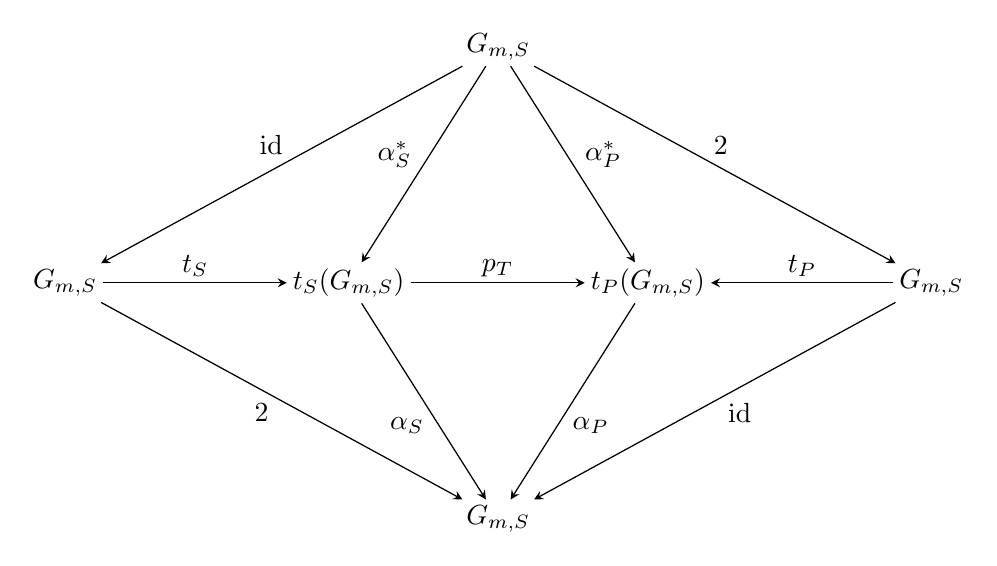
\begin{tikzpicture}[>=stealth,
  every node/.style={inner sep=2pt},
  every path/.style={line width=.45pt}]
  \node (top) at (0,3.0) {$\mathbb G_{m,S}$};
  \node (left) at (-5.5,0) {$\mathbb G_{m,S}$};
  \node (ts) at (-1.9,0) {$t_S(\mathbb G_{m,S})$};
  \node (tp) at (1.9,0) {$t_P(\mathbb G_{m,S})$};
  \node (right) at (5.5,0) {$\mathbb G_{m,S}$};
  \node (bottom) at (0,-3.0) {$\mathbb G_{m,S}$};

  \draw[->] (top) -- node[pos=.48,above left] {$\mathrm{id}$} (left);
  \draw[->] (top) -- node[pos=.55,above left] {$\alpha_S^\ast$} (ts);
  \draw[->] (top) -- node[pos=.55,above right] {$\alpha_P^\ast$} (tp);
  \draw[->] (top) -- node[pos=.48,above right] {$2$} (right);

  \draw[->] (left) -- node[above] {$t_S$} (ts);
  \draw[->] (ts) -- node[above] {$p_T$} (tp);
  \draw[->] (right) -- node[above] {$t_P$} (tp);

  \draw[->] (left) -- node[pos=.48,below left] {$2$} (bottom);
  \draw[->] (ts) -- node[pos=.55,below left] {$\alpha_S$} (bottom);
  \draw[->] (tp) -- node[pos=.55,below right] {$\alpha_P$} (bottom);
  \draw[->] (right) -- node[pos=.48,below right] {$\mathrm{id}$} (bottom);
\end{tikzpicture}
\end{center}
Its central portion is the commutative diagram of \SGARefLink{sga3:xx:4.1}{4.1}
\footnote{With \(q=1\).}
associated with the canonical morphism
\(p\circ i\colon\mathrm{SL}_L\to\mathrm P_L\), which induces a
morphism between the preceding elementary \(S\)-systems.

% Authority: Exp20-13oct24.pdf, section 5.1 through 5.6.

% END inputs/XX/tex/components/13_expose_XX_section5_par51_through_par56_en.tex

% BEGIN inputs/XX/tex/components/14_expose_XX_par57_through_theorem511_en.tex
\paragraph{\textbf{5.7.}}
\SGARefTarget{sga3:xx:5.7}
Let \((G,T,\alpha)\) now be an arbitrary elementary \(S\)-system.
Consider the commutative diagram
\begin{center}
\begin{tikzpicture}[>=stealth,
  every node/.style={inner sep=2pt},
  every path/.style={line width=.45pt}]
  \node (top) at (0,2.9) {$\mathbb G_{m,S}$};
  \node (left) at (-3.7,0) {$\mathbb G_{m,S}$};
  \node (mid) at (0,0) {$T$};
  \node (right) at (3.7,0) {$\mathbb G_{m,S}$};
  \node (bottom) at (0,-2.9) {$\mathbb G_{m,S}$};

  \draw[->] (top) -- node[pos=.48,above left] {$\mathrm{id}$} (left);
  \draw[->] (top) -- node[left] {$\alpha^\ast$} (mid);
  \draw[->] (top) -- node[pos=.48,above right] {$2$} (right);
  \draw[->] (left) -- node[above] {$\alpha^\ast$} (mid);
  \draw[->] (mid) -- node[above] {$\alpha$} (right);
  \draw[->] (left) -- node[pos=.48,below left] {$2$} (bottom);
  \draw[->] (mid) -- node[left] {$\alpha$} (bottom);
  \draw[->] (right) -- node[pos=.48,below right] {$\mathrm{id}$} (bottom);
\end{tikzpicture}
\end{center}
Combining this diagram with that of \SGARefLink{sga3:xx:5.6}{5.6} gives a commutative diagram
\begin{center}
\begin{tikzpicture}[>=stealth,
  every node/.style={inner sep=2pt},
  every path/.style={line width=.45pt}]
  \node (top) at (0,2.9) {$\mathbb G_{m,S}$};
  \node (left) at (-4.8,0) {$t_S(\mathbb G_{m,S})$};
  \node (mid) at (0,0) {$T$};
  \node (right) at (4.8,0) {$t_P(\mathbb G_{m,S})$};
  \node (bottom) at (0,-2.9) {$\mathbb G_{m,S}$};

  \draw[->] (top) -- node[pos=.5,above left] {$\alpha_S^\ast$} (left);
  \draw[->] (top) -- node[left] {$\alpha^\ast$} (mid);
  \draw[->] (top) -- node[pos=.5,above right] {$\alpha_P^\ast$} (right);
  \draw[->] (left) -- node[above] {$\alpha^\ast\circ t_S^{-1}$} (mid);
  \draw[->] (mid) -- node[above] {$t_P\circ\alpha$} (right);
  \draw[->] (left) -- node[pos=.5,below left] {$\alpha_S$} (bottom);
  \draw[->] (mid) -- node[left] {$\alpha$} (bottom);
  \draw[->] (right) -- node[pos=.5,below right] {$\alpha_P$} (bottom);
\end{tikzpicture}
\end{center}
Using \SGARefLink{sga3:xx:4.1}{4.1}, one obtains:

\paragraph{\textbf{Proposition 5.8.}}
\SGARefTarget{sga3:xx:5.8}
\emph{Let \(S\) be a scheme and let \((G,T,\alpha)\) be an
elementary \(S\)-system.  Put \(L=\mathfrak g^\alpha\), so that
\(L^{-1}=\mathfrak g^{-\alpha}\).}

\emph{\textup{(i)} There exists a unique group morphism
\(f\colon\mathrm{SL}_L\to G\) satisfying the following equivalent
conditions:}
\[
\begin{array}{ll}
\textup{(a)}
&
f\begin{pmatrix}z&0\\0&z^{-1}\end{pmatrix}=\alpha^\ast(z),
\qquad
f\begin{pmatrix}1&X\\0&1\end{pmatrix}=\exp(X);
\\[1.1em]
\textup{(b)}
&
f\begin{pmatrix}1&X\\0&1\end{pmatrix}=\exp(X),
\qquad
f\begin{pmatrix}1&0\\Y&1\end{pmatrix}=\exp(Y);
\\[1.1em]
\textup{(c)}
&
f\begin{pmatrix}1&X\\0&1\end{pmatrix}=\exp(X),
\qquad
f\begin{pmatrix}0&X\\-X^{-1}&0\end{pmatrix}=w_\alpha(X).
\end{array}
\]

\emph{\textup{(ii)} There exists a unique group morphism
\(g\colon G\to\mathrm P_L\) satisfying}
\[
 g(t)=
 \begin{pmatrix}\alpha(t)&0\\0&1\end{pmatrix},
 \qquad
 g(\exp(X))
 =p\begin{pmatrix}1&X\\0&1\end{pmatrix}.
\]
\emph{Moreover,}
\[
 g(\exp(Y))
 =p\begin{pmatrix}1&0\\Y&1\end{pmatrix},
 \qquad
 g(w_\alpha(X))
 =p\begin{pmatrix}0&X\\-X^{-1}&0\end{pmatrix}.
\]
\emph{The morphism \(g\) is faithfully flat and quasi-compact, with}
\[
 \Ker(g)=\Ker(\alpha)=\operatorname{Centr}(G),
\]
\emph{and \(g\circ f\) is the canonical morphism
\(\mathrm{SL}_L\to\mathrm P_L\).}

Notice that condition \textup{(b)} in \textup{(i)} gives an explicit
description of the duality between
\(\mathfrak g^\alpha\) and \(\mathfrak g^{-\alpha}\).

\paragraph{\textbf{Corollary 5.9.}}
\SGARefTarget{sga3:xx:5.9}
\emph{Let \((G,T,\alpha)\) be an elementary \(S\)-system.  The
subgroups}
\[
 T\cdot U_\alpha,\qquad T\cdot U_{-\alpha},
 \qquad U_\alpha,\qquad U_{-\alpha}
\]
\emph{are closed.}

Since \(U_\alpha\) is a closed subgroup scheme of
\(T\cdot U_\alpha\), it suffices to prove the assertion for the
latter.  By Noether's theorem \textup{(\SGARefLink{sga3:iv:proposition:5:3:1}{Exposé IV, 5.3.1} and \SGARefLink{sga3:iv:lemma:6:4:1}{6.4.1})},
it is enough to show that
\[
 (T\cdot U_\alpha)/\Ker(\alpha)
\]
is a closed subgroup of \(G/\Ker(\alpha)\).  By \SGARefLink{sga3:xx:5.8}{5.8}, this reduces to
the evident fact that the subgroup of \(\mathrm P_L\) defined by
\(c=0\) is closed; one may equivalently work in \(\mathrm{GL}_L\),
by another application of Noether's theorem.  Consequently, the
exponential morphisms of \SGARefLink{sga3:xx:1.5}{Theorem 1.5}\textup{(i)} are closed
immersions.

\smallskip
\noindent\textbf{N.B.}\ The corollary also follows from the fact that
\(T\cdot U_\alpha\) and \(T\cdot U_{-\alpha}\) are ``Borel
subgroups'' of \(G\) \textup{(cf.\ \SGARefLink{sga3:xii:7.10}{Exposé XII, 7.10})}.

\paragraph{\textbf{5.10.}}
\SGARefTarget{sga3:xx:5.10}
Let \(L\) be an invertible \(\mathcal O_S\)-module, and let
\[
 \mathbb G_{m,S}\xrightarrow{\ \alpha^\ast\ }T
 \xrightarrow{\ \alpha\ }\mathbb G_{m,S}
\]
be a diagram of groups, where \(T\) is a torus,\footnote{This
qualification is supplied by the editors.} such that
\(\alpha\circ\alpha^\ast=2\).  Let \(R\) be the maximal torus of
\(\Ker(\alpha)\), and put \(K=\alpha^{\ast-1}(R)\).  Then \(K\) is a
subgroup of multiplicative type of \(\mathbb G_{m,S}\); since
\(\alpha\circ\alpha^\ast=2\), it is even a subgroup of
\(\mu_{2,S}\).  In particular,
\[
 K\longrightarrow\mathrm{SL}_L,
 \qquad
 z\longmapsto\begin{pmatrix}z&0\\0&z^{-1}\end{pmatrix}
\]
is central.  Hence there is a central group monomorphism
\[
 K\longrightarrow R\times\mathrm{SL}_L,
 \qquad
 z\longmapsto
 \left(
 \alpha^\ast(z),
 \begin{pmatrix}z&0\\0&z^{-1}\end{pmatrix}
 \right).
\]

Let
\[
 G=(R\times\mathrm{SL}_L)/K.
\]
This is an affine smooth group over \(S\), with connected fibers.
The sequence
\[
 1\longrightarrow K\longrightarrow
 R\times t_S(\mathbb G_{m,S})
 \xrightarrow{\ u\ }T\longrightarrow1,
 \qquad
 u(x,t_S(z))=x\alpha^\ast(z),
\]
is exact.  The image of \(R\times t_S(\mathbb G_{m,S})\) in \(G\)
is therefore a torus \(T'\) isomorphic to \(T\).  If \(\alpha'\) is
the character of \(T'\) transported from \(\alpha\), one readily
checks that \((G,T',\alpha')\) is an elementary \(S\)-system, that
\(\mathfrak g^{\alpha'}\) is isomorphic to \(L\), and that
\(\alpha'^\ast\) is obtained from \(\alpha^\ast\) under the
isomorphism \(T\xrightarrow{\sim}T'\).  Thus the object
\[
 \left(
 \mathbb G_{m,S}\xrightarrow{\ \alpha'^\ast\ }T'
 \xrightarrow{\ \alpha'\ }\mathbb G_{m,S},\,
 \mathfrak g^{\alpha'}
 \right)
\]
of the category \(\mathcal D\) defined in \SGARefLink{sga3:xx:4.2}{4.2} is isomorphic to
\[
 \left(
 \mathbb G_{m,S}\xrightarrow{\ \alpha^\ast\ }T
 \xrightarrow{\ \alpha\ }\mathbb G_{m,S},\,L
 \right).
 \]
We have therefore proved:

\paragraph{\textbf{Theorem 5.11.}}
\SGARefTarget{sga3:xx:5.11}
\emph{With the notation of \SGARefLink{sga3:xx:4.2}{4.2}, the functor}
\[
 (G,T,\alpha)\longmapsto
 \left(
 \mathbb G_{m,S}\xrightarrow{\ \alpha^\ast\ }T
 \xrightarrow{\ \alpha\ }\mathbb G_{m,S},\,
 \mathfrak g^\alpha
 \right)
\]
\emph{is an equivalence of categories between
\(\mathcal E\) and \(\mathcal D\).}

% Authority: Exp20-13oct24.pdf, section 5.7 through theorem 5.11.

% END inputs/XX/tex/components/14_expose_XX_par57_through_theorem511_en.tex

% BEGIN inputs/XX/tex/components/15_expose_XX_section6_through_lemma621_en.tex
\section{Generators and Relations for an Elementary System}

\paragraph{\textbf{6.1.}}
\SGARefTarget{sga3:xx:6.1}
Let \(S\) be a scheme and let \((G,T,\alpha)\) be an elementary
\(S\)-system.  Let
\[
 X\in W(\mathfrak g^\alpha)^\times(S),
 \qquad u=\exp(X).
\]
As observed in \SGARefLink{sga3:xx:3.8}{3.8}, the element \(w=w_\alpha(X)\) satisfies, in
particular,
\[
 (wu)^3=e.
\]
\footnote{The editors added the sentence that follows.}
Let \(s_\alpha\) denote the automorphism of \(T\) induced by
\(\intaut(w)\).  By \SGARefLink{sga3:xx:3.1}{Theorem 3.1}\textup{\SGARefLink{sga3:xx:3.1:item:iii}{(iii)}}, for every \(S'\to S\)
and every \(t\in T(S')\),
\[
 s_\alpha(t)=\intaut(w)(t)
 =t\,\alpha^\ast\bigl(\alpha(t)^{-1}\bigr).
\]

\paragraph{\textbf{Theorem 6.2.}}
\SGARefTarget{sga3:xx:6.2}
\emph{Let \(H\) be a sheaf of groups over \(S\) for the fppf
topology.  Let}
\[
 f_T\colon T\longrightarrow H,
 \qquad
 f_\alpha\colon U_\alpha\longrightarrow H
\]
\emph{be group morphisms, and let \(h\in H(S)\).  There exists a
\textup{(necessarily unique)} group morphism}
\[
 f\colon G\longrightarrow H
\]
\emph{extending \(f_T\) and \(f_\alpha\) and satisfying \(f(w)=h\)
if and only if the following conditions hold:}

\emph{\textup{(i)} For every \(S'\to S\),
\(t\in T(S')\), and \(x\in U_\alpha(S')\),}
\begin{equation}
\tag{1}\label{sga3:xx:theorem:6-2:equation:1}
 f_T(t)f_\alpha(x)f_T(t)^{-1}
 =f_\alpha(txt^{-1})
 =f_\alpha\bigl(x^{\alpha(t)}\bigr).
\end{equation}
\emph{Equivalently, \(f_T\) and \(f_\alpha\) extend to a group
morphism \(T\cdot U_\alpha\to H\).}

\emph{\textup{(ii)} For every \(S'\to S\) and \(t\in T(S')\),}
\begin{equation}
\tag{2}\label{sga3:xx:theorem:6-2:equation:2}
 h f_T(t)h^{-1}
 =f_T(s_\alpha(t))
 =f_T\!\left(t\,\alpha^\ast(\alpha(t)^{-1})\right).
\end{equation}

\emph{\textup{(iii)} The following two relations hold in \(H(S)\):}
\begin{equation}
\tag{3}\label{sga3:xx:theorem:6-2:equation:3}
 h^2=f_T\bigl(\alpha^\ast(-1)\bigr),
\end{equation}
\begin{equation}
\tag{4}\label{sga3:xx:theorem:6-2:equation:4}
 \bigl(hf_\alpha(u)\bigr)^3=e.
\end{equation}

\smallskip
\noindent\emph{Proof.}
Write the laws on \(U_\alpha\) and \(U_{-\alpha}\) additively, while
writing their vector-space structures multiplicatively.  If \(f\)
has the asserted properties, then for
\(y\in U_{-\alpha}(S')\) one necessarily has
\[
 f(y)
 =f(w^{-1}wyw^{-1}w)
 =h f_\alpha(w^{-1}yw)h^{-1}.
\]
Define a morphism \(f_{-\alpha}\colon U_{-\alpha}\to H\) by
\begin{equation}
\tag{\(\ast_1\)}\label{sga3:xx:theorem:6-2:equation:ast-1}
 f_{-\alpha}(y)=h f_\alpha(w^{-1}yw)h^{-1}.
\end{equation}
It is a group morphism.  On the big cell \(\Omega\), the morphism
\(f\) is forced to satisfy
\[
 f(ytx)=f_{-\alpha}(y)f_T(t)f_\alpha(x).
\]
This proves uniqueness.  The conditions in the statement are
manifestly necessary; let us prove that they are sufficient.

Relation \textup{\SGARefLink{sga3:xx:theorem:6-2:equation:4}{(4)}} gives
\[
 h f_\alpha(u)h^{-1}h^2
 =
 f_\alpha(-u)h^{-1}f_\alpha(-u).
\]
By \textup{\SGARefLink{sga3:xx:theorem:6-2:equation:3}{(3)}} and \textup{\SGARefLink{sga3:xx:theorem:6-2:equation:1}{(1)}},
\(h^2=f_T(\alpha^\ast(-1))\) commutes with \(f_\alpha(-u)\), and
hence
\[
 h f_\alpha(u)h^{-1}
 =
 f_\alpha(-u)h f_\alpha(-u).
\]
By definition,
\[
 h f_\alpha(u)h^{-1}=f_{-\alpha}(wuw^{-1}),
\]
whereas \SGARefLink{sga3:xx:3.7}{3.7} gives
\begin{equation}
\tag{\(\ast_2\)}\label{sga3:xx:theorem:6-2:equation:ast-2}
 wuw^{-1}=-\widetilde u,
\end{equation}
with \(\widetilde u\) the element paired with \(u\).  Therefore
\begin{equation}
\tag{\(\ast_3\)}\label{sga3:xx:theorem:6-2:equation:ast-3}
 f_{-\alpha}(-\widetilde u)
 =
 f_\alpha(-u)h f_\alpha(-u).
\end{equation}

Let \(t\) be a section of \(T\) over a variable \(S'\to S\).
Apply \(\intaut(f_T(t))\) to this identity.  On the left one
obtains\footnote{The editors corrected the calculation that follows.}
\[
\begin{aligned}
 f_T(t)f_{-\alpha}(-\widetilde u)f_T(t)^{-1}
 &=
 f_T(t)h f_\alpha(u)h^{-1}f_T(t)^{-1}\\
 &=
 h\bigl(h^{-1}f_T(t)h\bigr)f_\alpha(u)
   \bigl(h^{-1}f_T(t)^{-1}h\bigr)h^{-1}\\
 &=
 h f_T(s_\alpha(t))f_\alpha(u)
   f_T(s_\alpha(t))^{-1}h^{-1}\\
 &=
 h f_\alpha\bigl(\alpha(s_\alpha(t))u\bigr)h^{-1}\\
 &=
 h f_\alpha\bigl(\alpha(t)^{-1}u\bigr)h^{-1}\\
 &=
 f_{-\alpha}\bigl(-\alpha(t)^{-1}\widetilde u\bigr).
\end{aligned}
\]
Here we used \textup{\SGARefLink{sga3:xx:theorem:6-2:equation:2}{(2)}}, \textup{\SGARefLink{sga3:xx:theorem:6-2:equation:1}{(1)}},
\(s_\alpha(t)=t\alpha^\ast(\alpha(t)^{-1})\), and
\(\alpha\circ\alpha^\ast=2\).

The right-hand side of \((\ast_3)\), after conjugation, becomes
\[
 f_\alpha(-\alpha(t)u)\,
 f_T(t)h f_T(t)^{-1}h^{-1}\,
 h f_\alpha(-\alpha(t)u).
\]
Since
\[
 h f_T(t)^{-1}h^{-1}
 =f_T(s_\alpha(t^{-1}))
  =f_T\bigl(t^{-1}\,\alpha^\ast(\alpha(t))\bigr),
\]
this equals
\[
 f_\alpha(-\alpha(t)u)\,
 f_T\bigl(\alpha^\ast(\alpha(t))\bigr)\,
 h f_\alpha(-\alpha(t)u).
\]
Comparison gives
\[
 f_{-\alpha}\bigl(-\alpha(t)^{-1}\widetilde u\bigr)
 =
 f_\alpha(-\alpha(t)u)\,
 f_T\bigl(\alpha^\ast(\alpha(t))\bigr)\,
 h f_\alpha(-\alpha(t)u).
\]
Since \(\alpha\colon T\to\mathbb G_{m,S}\) is faithfully flat and
\(H\) is a separated presheaf, \(-\alpha(t)^{-1}\) may be replaced
by an arbitrary section of \(\mathbb G_{m,S}\).  Thus:

\paragraph{\textbf{Lemma 6.2.1.}}
\SGARefTarget{sga3:xx:6.2.1}
\emph{For every \(S'\to S\) and every
\(z\in\mathbb G_m(S')\),}
\[
 f_{-\alpha}(z\widetilde u)
 =
 f_\alpha(z^{-1}u)\,
 f_T\bigl(\alpha^\ast(-z^{-1})\bigr)\,
 h f_\alpha(z^{-1}u).
\]

% Authority: Exp20-13oct24.pdf, section 6 through lemma 6.2.1.

% END inputs/XX/tex/components/15_expose_XX_section6_through_lemma621_en.tex

% BEGIN inputs/XX/tex/components/16_expose_XX_lemma622_through_end_en.tex
Let \(x,y\in\mathbb G_a(S')\), where \(S'\to S\), and suppose that
\(y\) and \(1+xy\) are invertible.  Applying \SGARefLink{sga3:xx:6.2.1}{Lemma 6.2.1} first with
\(z=y\), one obtains\footnote{The editors expanded the calculations
that follow.}
\[
 f_\alpha(xu)f_{-\alpha}(y\widetilde u)
 =
 f_\alpha\bigl((x+y^{-1})u\bigr)\,
 f_T\bigl(\alpha^\ast(-y^{-1})\bigr)\,
 h f_\alpha(y^{-1}u).
\]
Now \(x+y^{-1}=y^{-1}(1+xy)\).  Applying the lemma with
\(z=y/(1+xy)\) gives
\[
\begin{aligned}
 f_\alpha\bigl((x+y^{-1})u\bigr)
 &=
 f_{-\alpha}\!\left(\frac{y}{1+xy}\widetilde u\right)
 f_\alpha\bigl(-(x+y^{-1})u\bigr)\\
 &\qquad{}\cdot h\,
 f_T\!\left(\alpha^\ast\!\left(-\frac{y}{1+xy}\right)\right).
\end{aligned}
\]
Substitution in the preceding identity yields
\[
\begin{aligned}
 f_\alpha(xu)f_{-\alpha}(y\widetilde u)
 &=
 f_{-\alpha}\!\left(\frac{y}{1+xy}\widetilde u\right)
 f_\alpha\bigl(-(x+y^{-1})u\bigr)h^{-1}\\
 &\qquad{}\cdot
 f_T\bigl(\alpha^\ast(1+xy)^{-1}\bigr)
 h f_\alpha(y^{-1}u).
\end{aligned}
\]
Since \(h^{-1}f_T(t)h=f_T(s_\alpha(t))\) by \textup{(2)}
\textup{(recall that \(s_\alpha^2=\operatorname{id}\))}, and
\(s_\alpha\circ\alpha^\ast=-\alpha^\ast\), this is
\[
\begin{aligned}
 f_{-\alpha}\!\left(\frac{y}{1+xy}\widetilde u\right)
 f_\alpha\bigl(-(x+y^{-1})u\bigr)
 f_T\bigl(\alpha^\ast(1+xy)\bigr)
 f_\alpha(y^{-1}u).
\end{aligned}
\]
For \(x'\in U_\alpha(S')\) and
\(z\in\mathbb G_m(S')\), one has
\[
 f_\alpha(x')f_T(\alpha^\ast(z))
 =
 f_T(\alpha^\ast(z))f_\alpha(z^{-2}x').
\]
Consequently,
\[
\begin{aligned}
 f_\alpha(xu)f_{-\alpha}(y\widetilde u)
 &=
 f_{-\alpha}\!\left(\frac{y}{1+xy}\widetilde u\right)
 f_T\bigl(\alpha^\ast(1+xy)\bigr)\\
 &\qquad{}\cdot
 f_\alpha\!\left(
 \left[
 -\frac{y^{-1}(1+xy)}{(1+xy)^2}+y^{-1}
 \right]u
 \right)\\
 &=
 f_{-\alpha}\!\left(\frac{y}{1+xy}\widetilde u\right)
 f_T\bigl(\alpha^\ast(1+xy)\bigr)
 f_\alpha\!\left(\frac{x}{1+xy}u\right).
\end{aligned}
\]
We have proved:

\paragraph{\textbf{Lemma 6.2.2.}}
\SGARefTarget{sga3:xx:6.2.2}
\emph{Let \(S'\to S\).  If
\(a\in U_\alpha(S')\), \(b\in U_{-\alpha}^\times(S')\), and
\(1+ab\in\mathbb G_m(S')\), then}
\[
 f_\alpha(a)f_{-\alpha}(b)
 =
 f_{-\alpha}\!\left(\frac{b}{1+ab}\right)
 f_T\bigl(\alpha^\ast(1+ab)\bigr)
 f_\alpha\!\left(\frac{a}{1+ab}\right).
\]

By schematic density, this formula remains valid for
\(b\in U_{-\alpha}(S')\), with \(1+ab\) invertible.  Define
\[
 f\colon\Omega\longrightarrow H,
 \qquad
 f(ytx)=f_{-\alpha}(y)f_T(t)f_\alpha(x).
\]
It follows at once from \SGARefLink{sga3:xx:6.2.2}{Lemma 6.2.2}, condition \SGARefLink{sga3:xx:6.2}{6.2}\textup{(i)}, and
formula \textup{(F')} of \SGARefLink{sga3:xx:2.4}{2.4} that whenever
\(g,g'\in\Omega(S')\) and \(gg'\in\Omega(S')\), one has
\[
 f(gg')=f(g)f(g').
\]
By \SGARefLink{sga3:xviii:prop:2.3}{Exposé XVIII, 2.3}\textup{\SGARefLink{sga3:xviii:prop:2.3:item:iii}{(iii)}} and \SGARefLink{sga3:xx:2.4}{2.4},\footnote{Each geometric
fiber of \(G\) is connected, for example by \SGARefLink{sga3:xx:section:1}{1.1}.} there is therefore
a group morphism \(G\to H\) extending \(f\).  Denote it again by
\(f\).  It remains only to prove that \(f(w_\alpha)=h\).  Since
\[
 w_\alpha=u\cdot(-\widetilde u)\cdot u,
\]
formula \((\ast_3)\) gives\footnote{The editors simplified the
original argument by invoking \((\ast_3)\).}
\[
 f(w_\alpha)
 =f_\alpha(u)f_{-\alpha}(-\widetilde u)f_\alpha(u)
 =h.
\]
This completes the proof of \SGARefLink{sga3:xx:6.2}{Theorem 6.2}.

\paragraph{\textbf{Remark 6.3.}}
\SGARefTarget{sga3:xx:6.3}
\emph{These results will be completed in \SGARefLink{sga3:xxiii:subsection:3-5}{Exposé XXIII, 3.5}.}

% Authority: Exp20-13oct24.pdf, lemma 6.2.2 through the end of Exposé XX.

% END inputs/XX/tex/components/16_expose_XX_lemma622_through_end_en.tex


